\documentclass[11pt]{article}
\usepackage{graphicx}
\usepackage[utf8]{inputenc} 
\usepackage{amsmath}
\usepackage{cancel}
\usepackage{bbold}
\usepackage{color}
\usepackage{amsfonts}
\usepackage{mathtools}
\usepackage{braket}
\usepackage{float}
\usepackage{lscape}
\usepackage{multicol}
\usepackage[compat=1.1.0]{tikz-feynman}
\usepackage{tikz}
\usepackage{subcaption}
\usepackage{multicol}

\usepackage{geometry}
\geometry{legalpaper, margin=1.0in}

\begin{document}
\title{Supersymmetry at the LHC}
\author{Ingrid A V Holm}
\maketitle

\pagebreak


\section*{Outline}
\begin{flushleft}
This project will contain the following
\begin{itemize}
\item A motivation for supersymmetry; what \textit{is} supersymmetry and what is the motivation for it? An introduction.
\item A calculation of the QCD production of squarks at the LHC, i.e. $qq' \rightarrow \tilde{q} \tilde{q}'$.
\item Calculate the NLO terms using Prospino \cite{beenakker1996prospino} and compare to the analytic calculation. What does this mean for the error in the cross section?
\item Compare with data (from ATLAS?) to look for jets or some process with final state leptons (not decided yet). 
\begin{align*}
\tilde{q} &\rightarrow q \tilde{\chi}_0^1\\
\tilde{q} &\rightarrow q' \tilde{\chi}_0^+ \rightarrow q' l \tilde{\chi}_0^1
\end{align*}
\end{itemize}
\end{flushleft}




\section{Why supersymmetry?}

\begin{flushleft}
The best description of subatomic physics we have is called the Standard Model of Particle Physics (SM), or the Standard Model for short. Its ability to predict experimental outcome has proven quite astonishing. The Standard Model is described by the symmetries under which the laws of nature remain unchanged. These can be translations or rotations in space, or more complicated symmetries such as the color symmetry of strong interactions. The symmetry group of the Standard Model is
\begin{align}
SU(3)_C \times SU(2)_W \times U(1)_Y,
\end{align}
where $SU(3)$ represents the strong interaction between quarks and gluons, i.e. the force that holds a proton together, and $SU(2) \times U(1)$ represents the electroweak interaction. The electroweak interaction is broken down to the weak and electromagnetic interactions at an energy scale around $246$ GeV. The weak interaction is responsible for radioactive decay, such as a neutron decaying into a proton, an electron and a neutrino. The electromagnetic interaction is perhaps more familiar, as it is responsible for electric and magnetic phenomena. Despite its success, the SM has some discrepancies. Of these the hierarchy problem -- the enormous difference in energy scales of the SM -- is one of the most severe.
\end{flushleft}

\subsection*{The Hierarchy Problem}
\begin{flushleft}
In order to fully understand the hierarchy problem, it's helpful to know how the elementary particles obtain their mass. The particles of the SM, which we divide into fermions and bosons according to their spin, get mass from the Higgs mechanism. The Higgs mechanism is essentially the Spontaneous Symmetry Breaking of the Higgs potential in a local gauge invariant theory. The Higgs boson is described by a 'mexican hat' potential, given by
\begin{align*}
V(|\phi|^2) = - \mu^2 |\phi|^2 + \lambda|\phi|^4.
\end{align*}
When the symmetry of this potential is spontaneously broken, the Higgs couples to particles, giving them mass due to the non-zero value of the vacuum expectation value. For a fermion $f$ (and its anti-particle $\bar{f}$) this yields an interaction term in the Lagrangian of the following form
\begin{align}
\Delta \mathcal{L} = - \frac{1}{2} \lambda_f H \bar{f}f,
\end{align}
where $\lambda_f \propto m_f$. So the coupling of particles to the Higgs is proportional to their mass. Now, the expectation value of the vacuum is non-zero, and this is connected to the production of pairs of \textit{virtual particles} 'form nothing'. These cannot be observed, but affect the measurements  of the various masses. Another consequence of vacuum fluctuations is the screening of electric charge, see Fig. (\ref{fig:: vacuum polarization}). Since the charge of an electron \textit{polarizes the vacuum}, the actual electric charge is screened, and we measure a lower value than the \textit{bare} charge (the charge you would hypothetically measure at zero distance from the electron). The further away from the electron you get (low energy scale) the lower charge you will measure.
\begin{figure}[H]
\centering
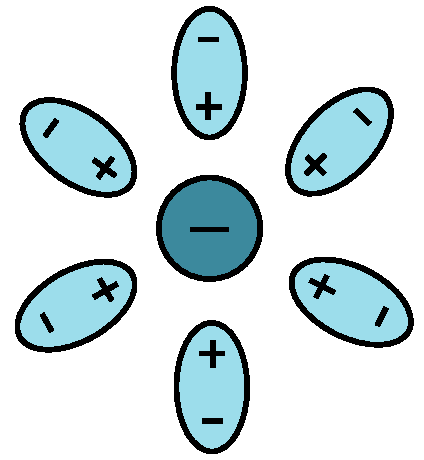
\includegraphics[scale=0.6]{vacuum_polarization.pdf}
\caption{Electric charge screening from vacuum polarization.}
\label{fig:: vacuum polarization}
\end{figure}

Calculating the scale dependence of a parameter of a theory is referred to as renormalization. Such parameters can be coupling constants, field strengths or masses. For the Higgs mass, some of the Feynman diagrams contributing to the mass term are
\begin{figure}[H]
\begin{flushleft}
\begin{tikzpicture}
\begin{feynman}
\vertex (p1); \vertex [below=1.1cm of p1, blob] (p2) {}; \vertex [below=3cm of p1] (p3); \vertex [below =5 cm of p1] (p4);

\node at (-4, -1.5) {The mass of the Higgs \(m^2\)};

\diagram{(p1) --[scalar, edge label={\(H\)}] (p2) -- [scalar, edge label={\(H\)}] (p3)};

\hspace{10mm}
\node at (0,-1.5) {=};
\hspace{17mm}

\vertex (s1); \vertex [below=1.3cm of s1] (s2); \vertex [below=3cm of s1] (s3); 

\node at (-0.8,-1.5) {\(i m_0^2\)};

\diagram{(s1) --[scalar, edge label={\(H\)}] (s2) --[scalar, edge label={\(H\)}] (s3)};

\hspace{10mm}
\node at (0,-1.5) {+};
\hspace{15mm}

\vertex (q1); \vertex [below=1.5cm of q1] (q2); \vertex [below=1.5cm of q2] (q3); \vertex [right= 0.8cm of q2] (ql2); 

\node at (-0.6,-1.5) {\(i \frac{\lambda}{\delta^2}\)};

\diagram{(q1) -- [scalar, edge label={\(H\)}](q2) -- [scalar, edge label={\(H\)}](q3), (q2) --[scalar, half left] (ql2) --[scalar, half left] (q2)};

\hspace{12mm}
\node at (0,-1.5) {+};
\hspace{17mm}

\vertex (r1); \vertex [below=1cm of r1] (r2); \vertex [below=1cm of r2] (r3); \vertex [below=2cm of r2] (r4);

\node at (-0.6,-1.5) {\(-i \frac{g^2}{\delta^2}\)};

\hspace{4mm}

\diagram{(r1) -- [scalar, edge label={\(H\)}](r2) -- [fermion, half left] (r3) -- [fermion, half left] (r2), (r3) -- [scalar, edge label={\(H\)}] (r4)};

\node at (1.2,-1.5) {+...};
\end{feynman}
\end{tikzpicture}

\end{flushleft}
\end{figure}
The mathematical expressions corresponding to the diagrams are to the left of each diagram. $\lambda$ is the coupling constant for the boson, while $g$ is the coupling constant for the fermion. The propagator of the Higgs is a sum of propagators with different loops attached to them. A propagator is the quantum mechanical way of summing up 'all the possible ways to get from state A to state B'. For the correction terms (terms with loops), the distance between connecting points is unknown, so we must integrate over all possible distances $\delta$.  Clearly the expression blows up as $\delta$ becomes very small. This can be somewhat mended by introducing a cutoff length scale. At the Planck scale gravity becomes comparable in strength to the other interactions. Since there is no way to explain gravity using the Standard Model, we don't really know what happens at this scale. Therefore we only integrate up to the Planck scale, which is about $\delta \simeq 10^{-25}$. Even with this cutoff the mass term is enormous. The Higgs mass has been experimentally measured at the LHC, and found to be around $125$ GeV. Yet, according to the SM it should be closer to $10^{19}$ GeV. How can we explain this enormous scale difference? This is the so called \textit{Hierarchy Problem}. 
\end{flushleft}

\begin{flushleft}
To get a feeling of how disastrous this problem is, thermodynamics provides a useful analogy. If you were to put a glass of water in flames, you would expect the water to become hot and even evaporate. Now imagine you put an ice cube in the flames, left, and came back ten minutes later -- you would certainly expect it to have melted. The ice \textit{could} be unaffected by the flames, but it would be very surprising. In the same way, it's ridiculously unlikely that the Higgs mass should stay at $125$ GeV.
\end{flushleft}

\begin{flushleft}
To explain this gap in the SM would require fine-tuning, or a very precise adjustment of the parameters of the theory. This is in general problematic since the mechanism responsible for the fine tuning is unknown. Naturalness is the rule that the parameters of a fundamental physical theory should not be too fine-tuned. However, fine tuning can be avoided by introducing additional symmetries.
\end{flushleft}

\subsection*{Supersymmetry}
\begin{flushleft}
A theory that offers a very elegant solution to the hierarchy problem is \textit{supersymmetry}. It also offers a way to unify the gauge symmetry couplings into a Grand Unifying theory, and provides a candidate for Dark Matter, but this will not be discussed here. Before diving into the technicalities, let's consider the difference between fermions and bosons, which lies at the heart of supersymmetry. Fermions are particles with half-integer spin that follow Fermi-Dirac statistics, meaning that they are antisymmetric under interchange of particles. Bosons have integer spin and follow Bose-Einstein statistics, which in turn means they are symmetric under interchange. Let's consider two fermion loops in the vacuum, which we can think of as the creation of a virtual pair of fermion and anti-fermion.

\begin{figure}[H]
\centering
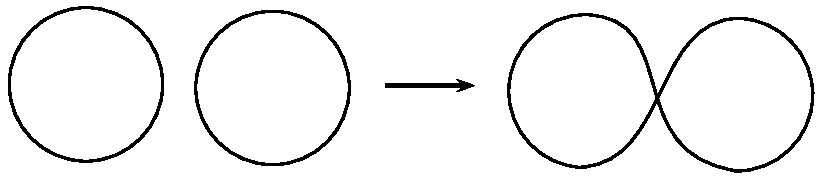
\includegraphics[scale=0.8]{fermion_loop.pdf}
\caption{Two fermion/boson loops merge into one loop.}
\label{fig:: fermion loop}
\end{figure}

If we move the loops very close together, we can imagine connecting them, turning them into one single loop, as shown in Fig. (\ref{fig:: fermion loop}). Because of the aforementioned Fermi statistics that govern fermions this interchange should give a minus sign. For bosons, however, the wavefunction is symmetric and no minus sign is needed. This is why fermion loops give a minus sign to an expression, while boson loops don't. Let's now return to the mass renormalization of the Higgs boson. A fermion loop would give a term for the Lagrangian of the following  form  
\begin{align}
\Delta \mathcal{L}_f \propto - \frac{g^2}{\delta^2},
\end{align}
while a boson would contribute with
\begin{align}
\Delta \mathcal{L}_b \propto \frac{\lambda}{\delta^2}.
\end{align}
If the coupling constants, and thereby the masses, were equal i.e. $\lambda = g^2$, these terms would cancel. That way the enormous correction would simply cancel out, and the measured value of the Higgs mass would fit with prediction. This is the essence of supersymmetry; introducing a symmetry between fermions and bosons with the exact same quantum numbers (apart from their spin).
\end{flushleft}
\begin{figure}[H]
\centering
\begin{tikzpicture}
\begin{feynman}
\vertex (p1); \vertex [below=2cm of p1] (p2); \vertex [below=2cm of p2] (p3); \vertex [right=1.5cm of p2] (p2r); \vertex [below=1cm of p1] (p2f); \vertex [below=2cm of p2f] (p3f); \vertex [below=1.cm of p3f] (p4f);

\diagram{
(p1) --[scalar, edge label={\(H\)}] (p2f); (p2f) --[fermion, half left, edge label={\(f\)}] (p3f), (p3f) --[fermion, half left, edge label={\(f\)}] (p2f), (p3f) --[scalar, edge label={\(H\)}] (p4f)
};

\hspace{3cm}

\diagram{
(p1) -- [scalar, edge label={\(H\)}] (p2), (p2) -- [half left] (p2r) -- [half left] (p2), (p2) -- [scalar, edge label={\(H\)}] (p3)
};
\end{feynman}
\end{tikzpicture}
\caption{Corrections to the Higgs mass. The diagram on the left is from SM, and on the right is the supersymmetric correction.}
\label{fig:: Higgs correction}
\end{figure}

\begin{flushleft}
Supersymmetry introduces so-called superpartners for all particles, which differ in spin by half a unit. Superpartners have not yet been observed, so their masses must be different from the SM particles, and so supersymmetry must be a broken symmetry. The particles along with their partners, the sparticles, comprise supermultiplets. Supersymmetry comes in many versions. Amongst the most common is the Minimal Supersymmetric extension of the Standard Model (MSSM). The supersymmetry transformation turns a fermion into a boson and vice versa, via the operator $Q$
\begin{align*}
Q \ket{\text{Boson}} = \ket{\text{Fermion}}, \text{ } Q \ket{\text{Fermion}} = \ket{\text{Boson}} 
\end{align*}
\begin{table}[H]
\centering
\title{\textbf{Field content of the MSSM}}

\begin{tabular}{|c|c|c|c|c|c|}
\hline
Supermultiplets & Bosonic fields & Fermionic partners & SU(3) & SU(2) & U(1)\\
\hline
gluon/gluino & $g$ & $\tilde{g}$ & 8 & 1 & 0\\
gauge/gaugino & $W^{\pm}$, $W^0$ & $\tilde{W}^{\pm}$, $\tilde{W}^0$ & 1 & 3 & 0\\
& $B$ & $\tilde{B}$ & 1 & 1 & 0\\
\hline
slepton/lepton & $(\tilde{\nu}_L, \tilde{e}_L^-)$ & $(\nu, e^-)_L$ & 1 & 2 & -1\\
& $\tilde{e}^+_R$ & $e^c_L$ & 1 & 1 & 2\\
\hline
squark/quark & $(\tilde{u}_L, \tilde{d}_L)$ & $(u,d)_L$ & 3 & 2 & 1/3\\
& $\tilde{u}*_R$ & $u^c_L$ & $\bar{3}$ & 1 & -4/3\\
& $\tilde{d}*_R$ & $d^c_L$ & $\bar{3}$ & 1 & 2/3\\
\hline
Higgs/higgsino & $(H^0_d, H^-_d)$ & $(\tilde{H}_d^0, \tilde{H}_d^-)$ & 1 & 2 & -1\\
& $(H_u^+, H^0_u)$ & $(\tilde{H}_u^+, \tilde{H}^0_u)$ & 1 & 2 & 1\\
\hline
\end{tabular}
\caption{The fermions and bosons that make the minimal supersymmetric extension of the Standard Model. }
\end{table}
\end{flushleft}

\begin{flushleft}
With supersymmetry another parity is introduced, namely the multiplicative $R$-parity. $R$-parity is $-1$ for supersymmetric particles and $1$ for SM particles. Invariance under $R$-parity requires that all supersymmetry vertices include 2 sparticles. This implies that sparticles decay into sparticles. There must therefore be a lightest, preferably color and electrically neutral, supersymmetric particle called the lightest neutralino $\tilde{\chi}^0_1$. This particle would behave like a heavy neutrino, and a typical signature for supersymmetric particles in a collider would be large missing transverse energy. Moreover, the neutralino is a good candidate for dark matter. It is protected from decay due to R-parity.
\end{flushleft}

\begin{flushleft}
In the SM we have one left-handed scalar Higgs doublet. In MSSM this doublet is promoted to a doublet of left-handed superfields which couple to up- and down-type fermions. The up-type Higgs $\hat{H}_u$ has weak hypercharge $Y=1$, and gives mass to up-type fermions. The down-type Higgs $\hat{H}_d$ has weak hypercharge $Y=-1$ and gives mass the to down-type fermions. This gives a new Higgs potential whose spontaneous breaking of electroweak symmetry requires two conditions
\begin{align*}
B &= \frac{(m_{H_d}^2-m^2_{H_u}) \tan 2 \beta + M_Z^2 \sin 2 \beta}{2 \mu},\\
\mu^2 &= \frac{m_{H_u}^2 \sin^2 \beta - m_{H_d}^2 \cos^2 \beta}{\cos 2 \beta} - \frac{M_Z^2}{2},
\end{align*}
where $\tan \beta \equiv v_u/v_d$ is the ratio of vacuum expectation values for the up- and down-type Higgs. For supersymmetric gravity-mediated SUSY breaking (SUGRA), this is one of five parameters, where the others are (1) a common mass for all scalar particles $m_0$; (2) a common gaugino mass $m_{1/2}$; (3) the trilinear Higgs-fermion-fermion coupling $A_0$; and (4) the sign of the higgsino mass parameter $sgn(\mu)$. The most recent exclusion limits on mSUGRA (an example of SUGRA) are given in Fig. (\ref{fig:: atlas msugra}). The search in this project would correspond to the (0+1)-lepton combination limit.
\end{flushleft}
\begin{figure}[H]
\centering
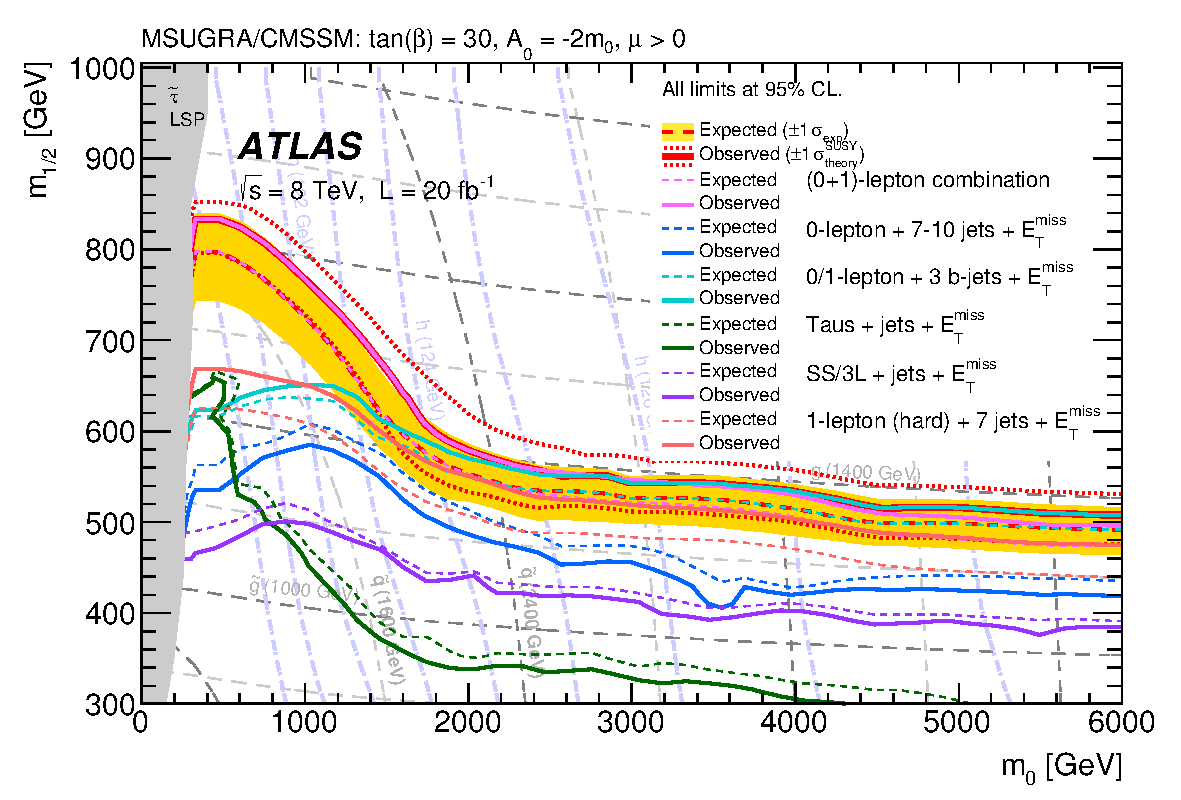
\includegraphics[scale=0.6]{plots/ATLAS_SUSY_MSUGRA.pdf}
\caption{$8$ TeV limits on SUGRA from ATLAS (2015).}
\label{fig:: atlas msugra}
\end{figure}

\begin{flushleft}
Section \textbf{1} gives a short motivation for and introduction to supersymmetry. In section \textbf{2} we've calculated analytically the leading order term of the cross section. Section \textbf{3} discusses the need for NLO terms, and introduces Prospino as a tool to calculate this. Section \textbf{4} looks for supersymmetry signals in the ATLAS OpenData. In section \textbf{5} the results can be found, and a short conclusion is given in Section \textbf{6}.
\end{flushleft}

\begin{figure}[H]
\centering
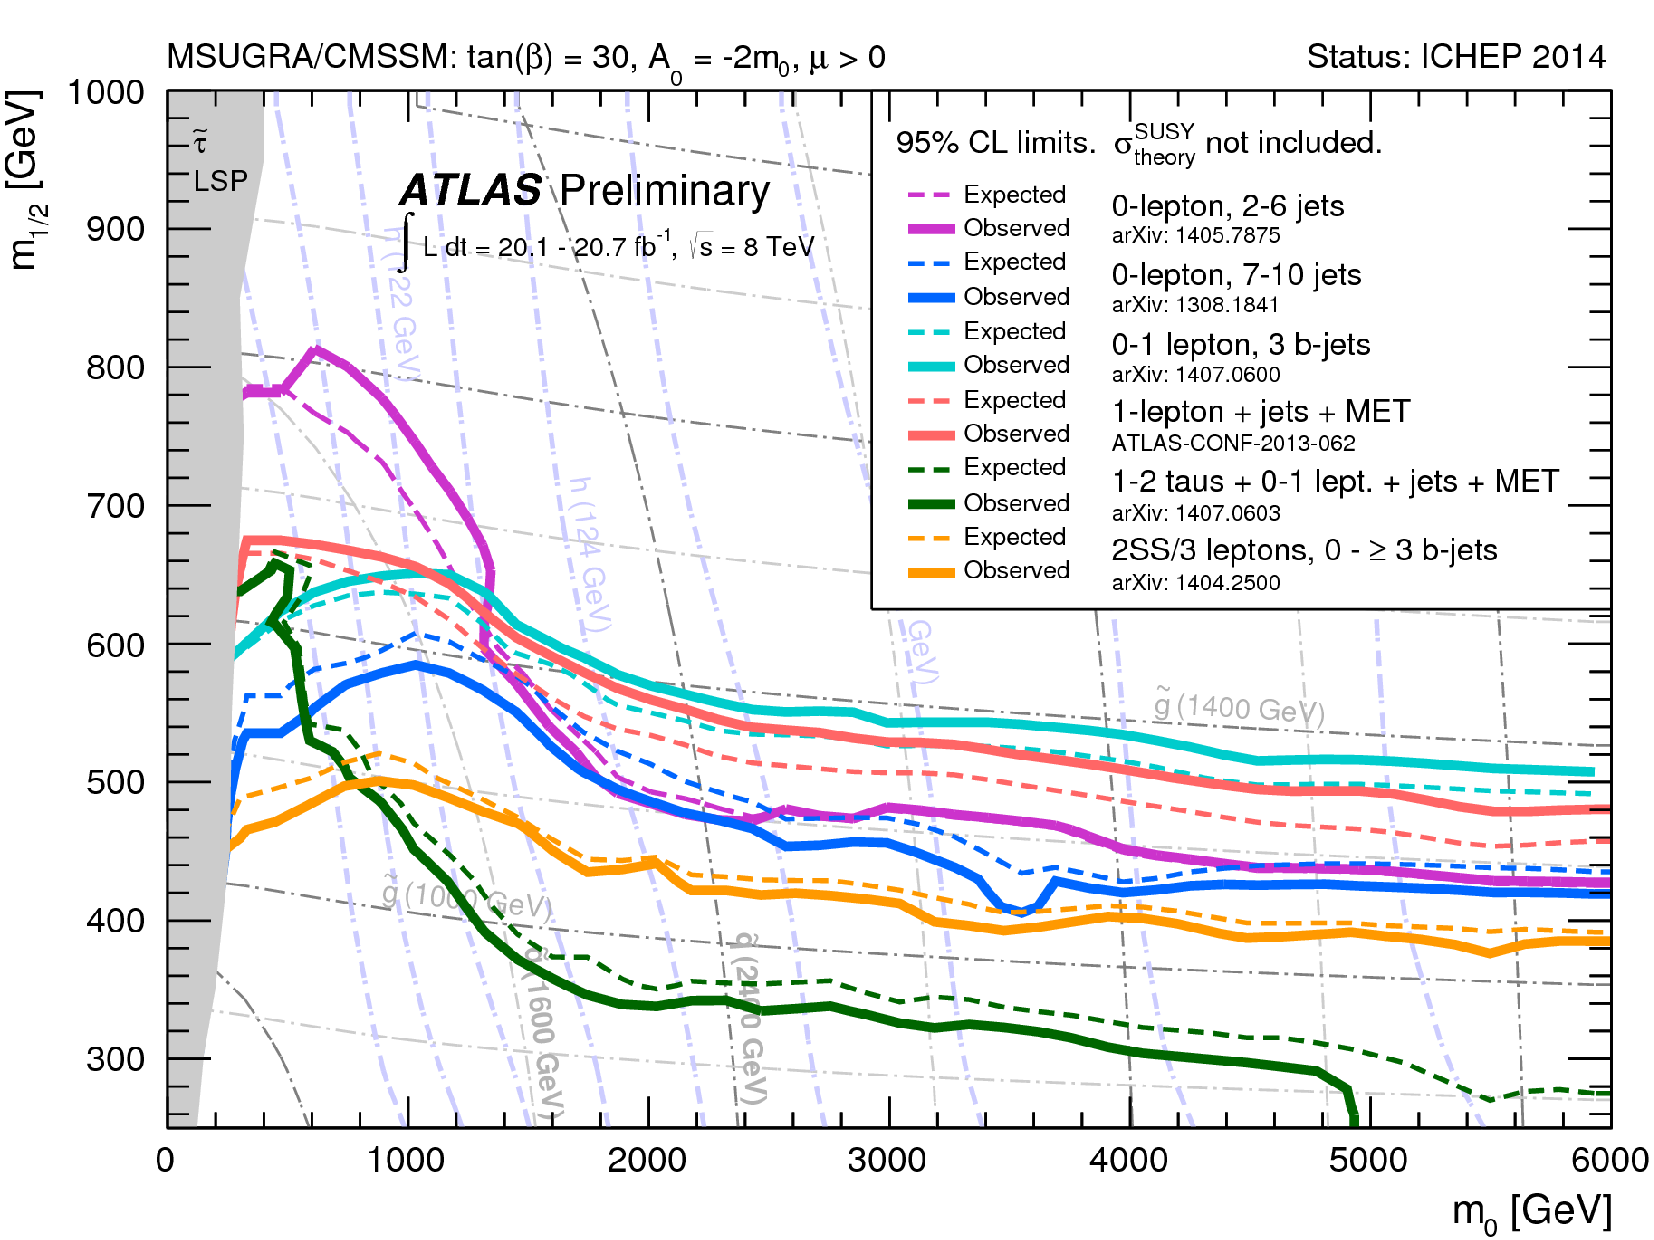
\includegraphics[scale=0.6]{atlas_preliminary.pdf}
\end{figure}


\section{QCD squark production}

\begin{flushleft}
A possible supersymmetric process to look for at the LHC is the production of squark-pairs. Squarks could be produced by colliding energetic protons, and the subsequent fusion of two quarks. Here we will calculate the leading order term of the cross section for this process, i.e. the probability of producing squarks through proton collision. The feynman diagram for the process 
\begin{align*}
qq \rightarrow \tilde{q} \tilde{q},
\end{align*}
is given in Fig. (\ref{fig::Feynman qq}). Here we consider the process via the strong interaction, as this is a likely channel at current LHC energies (13 TeV). The total matrix element gets a contribution from the $t$- and $u$-channel.
\begin{figure}[H]
\centering
\begin{tikzpicture}
\begin{feynman}
\vertex (p1) {\(q_i\)}; \vertex [right= of p1] (s1); \vertex [right= of s1] (q1){\(\tilde{q}_i\)}; \vertex [below=of p1] (p2) {\(q_j\)}; \vertex [right=of p2] (s2) ; \vertex [right= of s2] (q2) {\(\tilde{q}_j\)} ;
\diagram{
(p1) --[fermion, momentum=\(k_1\)] (s1) -- [scalar, momentum=\(p_1\)] (q1), (s1)-- [gluon] (s2) -- (s1), (p2) --[fermion, momentum=\(k_2\)] (s2) --[scalar, momentum=\(p_2\)] (q2)
};
\end{feynman}
\end{tikzpicture}
\begin{tikzpicture}
\begin{feynman}
\vertex (p1) {\(q_i\)}; \vertex [right= of p1] (s1); \vertex [right= of s1] (q1){\(\tilde{q}_i\)}; \vertex [below=of p1] (p2) {\(q_j\)}; \vertex [right=of p2] (s2) ; \vertex [right= of s2] (q2) {\(\tilde{q}_j\)} ;
\diagram{
(p1) --[fermion] (s1) -- [scalar] (q2), (s1)-- [gluon] (s2) -- (s1), (p2) --[fermion] (s2) --[scalar] (q1)
};
\end{feynman}
\end{tikzpicture}
\caption{Feynman diagrams for squark pair production in quark quark collisions, both $t$ and $u$ diagram. Notice that the u-channel (right diagram) is only possible for $i=j$.}
\label{fig::Feynman qq}
\end{figure}
The momentum of the gluino is denoted $p$ in the calculations, and defined as $p= k_2-p_2 $ for the $t$-channel and $p=k_2-p_1$ for the $u$-channel. The chiralitites are decided later, and are simply denoted as $P$ and $P'$ for now. A more detailed calculation can be found in Appendix A. The expression for the matrix element of the pure $t$-channel becomes (reading direction is from $q_j$ to $q_i$)
\begin{align*}
i \mathcal{M} &= \bar{v} (k_1) \Big( -i \sqrt{2} g P (t_a)^{ij}\Big) \times \delta^{ab} \frac{i}{\cancel{p} - m_{\tilde{g}}} \times \Big( -i \sqrt{2} gP'(t_b)^{lk} \Big) \times u(k_2)\\
&= - \frac{i 2 g^2}{p^2 - m_{\tilde{g}}^2 + i \epsilon}\big( \bar{v} (k_1)  P (t_a)^{ij}(\cancel{p} + m_{\tilde{g}}) P'(t^a)^{lk} u(k_2) \big)\\
&= - (t_a)^{ij}(t^a)^{lk} \times \frac{i 2 g^2}{t_g^2} \times  \bar{v} (k_1)  P (\cancel{p} + m_{\tilde{g}}) P' u(k_2) ,
\end{align*}
where the color factor has been factored out. The charge conjugate matrix element
\begin{align*}
i \mathcal{\bar{M}} & = (t_a)^{ij}(t^a)^{lk} \times \frac{i 2 g^2}{t_g^2} \times \bar{u} (k_2)  P (\cancel{p} + m_{\tilde{g}}) P' v(k_1) .
\end{align*}
Some Mandelstam variables have been used to clean up the expresson; $t= p^2 = (k_2 - p_2)^2$, $t_g = t - m_{\tilde{g}}^2$. The matrix element squared is then
\begin{align*}
|\mathcal{M}_t|^2 &=  (t_a)^{ij} (t^a)^{lk} (t_b)^{mn} (t^b)^{op} \times \frac{4 g^4}{t_g^2}
\big( \bar{v} (k_1)  P (\cancel{p} + m_{\tilde{g}}) P' u(k_2) \big)
\big( \bar{u} (k_2)  P (\cancel{p} + m_{\tilde{g}}) P' v(k_1) \big)
\end{align*}
Now average over spin
\begin{align*}
\sum |\mathcal{M}|^2 &= A_{color, t} \times \frac{4 g^4}{t_g^2} \text{tr} \big[ 
\cancel{k}_1 P (\cancel{p} + m_{\tilde{g}}) P' \cancel{k}_2 P (\cancel{p} + m_{\tilde{g}}) P' \big],
\end{align*}
where $A_{color, t}= (t_a)^{ij} (t^a)^{lk} (t_b)^{mn} (t^b)^{op}$. Since the quark mass is small compared to $m_g$, $m_{\tilde{q}}$ and $m_{\tilde{g}}$, we've set $m_q=0$.
At this point we need to consider the different combinations of chiralities. The traces for the different cases are
\begin{center}
\textit{Different chiralities }$P=P_{R/L}$, $P'=P_{L/R}$
\end{center}
\begin{align*}
\text{tr} \big[ 
\cancel{k}_1 P_{R/L} (\cancel{p} + m_{\tilde{g}}) P_{L/R} \cancel{k}_2 P_{R/L} (\cancel{p} + m_{\tilde{g}}) P_{L/R} \big]
&= 2 \big(
2 (p \cdot k_2) (k_1 \cdot p) - p^2 (k_1 \cdot k_2)\big).
\end{align*}

\begin{center}
\textit{Equal chiralities} $P=P_{R/L}$, $P'=P_{R/L}$
\end{center}
\begin{align*}
\text{tr} \big[ 
\cancel{k}_1 P_{R/L} (\cancel{p} + m_{\tilde{g}}) P_{R/L} \cancel{k}_2 P_{R/L} (\cancel{p} + m_{\tilde{g}}) P_{R/L} \big]&= 2  m_{\tilde{g}}^2 (k_1 \cdot k_2)
\end{align*}
where we've used that $P_{R/L}P_{R/L} = P_{R/L}$, $(\gamma^5)^2 = 1$ and $\text{tr}[\gamma^5 \gamma^{\mu} \gamma^{\nu}]=0$. In terms of the Mandelstam variables, which are here defined as
\begin{multicols}{3}

\begin{align*}
s &= (k_1 + k_2)^2 = 2 k_1 \cdot k_2\\
t &= (k_2-p_2)^2 = m_{\tilde{q}}^2 - 2 (k_2 \cdot p_2),\\
u &= (k_1 - p_2)^2 = m_{\tilde{q}}^2 - 2 (k_1 \cdot p_2),
\end{align*}

\begin{align*}
t_1 &= (k_2-p_2)^2 - m_{\tilde{q}}^2,\\
u_1 &= (k_1-p_2)^2 - m_{\tilde{q}}^2,
\end{align*}

\begin{align*}
t_g &= (k_2-p_2)^2 - m_{\tilde{g}}^2,\\
u_g &= (k_1-p_2)^2 - m_{\tilde{g}}^2,
\end{align*}

\end{multicols}
the expression is simplified to
\begin{align*}
&2(2 (p \cdot k_2) (k_1 \cdot p) - p^2 (k_1 \cdot k_2) ) + 2m_{\tilde{g}}^2 (k_1 \cdot k_2) =  2 \big[t_1u_1 -s(m_{\tilde{q}}^2 - m_{\tilde{g}}^2) \big].
\end{align*}
Note that for equal quark flavors, the two possibilities for different chiralities are in fact equal, and so there should be a factor of $1/2$ there. Now put this back into the expression 
\begin{align*}
\sum |\mathcal{M}|^2 &=   (t_a)^{ij} (t^a)^{lk} (t_b)^{mn} (t^b)^{op}  \times\frac{4 g^4}{t_g^2} \Big[\delta_{ij} \big(\frac{1}{2}(t_1u_1 -sm_{\tilde{q}}^2)+  sm_{\tilde{g}}^2 \big) + (1-\delta_{ij})\big(t_1u_1 -s(m_{\tilde{q}}^2- m_{\tilde{g}}^2) \big)\Big].
\end{align*}
The color factor is
\begin{align*}
(t^a)^{ij}(t_a)^{kl}(t^b)_{ij}(t_b)^{kl} = \frac{1}{2}NC_F,
\end{align*}
where we have defined $C_F = \frac{N^2 -1}{2}$. Adding a factor $2$ because we are summing over the different chiralities, the full expression for the $t$-channel is then
\begin{align*}
\sum |\mathcal{M}_t|^2 &= NC_F \frac{4g^4}{t_g^2} \Big[ \delta_{ij} \big(\frac{1}{2}(t_1u_1-sm_{\tilde{q}}^2) + sm_{\tilde{g}}^2 \big) + (1-\delta_{ij}) \big(t_1u_s - s(m_{\tilde{q}}^2 - m_{\tilde{g}}^2) \big)\Big]
\end{align*}
\end{flushleft}

\begin{flushleft}
The expression for the $u$-channel diagram is identical, except the exchange of $t_g^2 \rightarrow u_g^2$, and it only contributes for $i =j$, so the matrix element is
\begin{align*}
\sum |\mathcal{M}_u|^2 &= \delta_{ij} NC_F \frac{4g^4}{u_g^2} \Big[ \frac{1}{2}(t_1u_1-sm_{\tilde{q}}^2) + sm_{\tilde{g}}^2 \Big]. 
\end{align*}
\end{flushleft}

\subsection*{Cross term}
\begin{flushleft}
The $ut$ cross term comes from
\begin{align*}
i \mathcal{M}_{ut} &= A_{color, ut}\frac{-i 2 g^2}{t_g}\big( \bar{v} (k_1)  P (\cancel{p} + m_{\tilde{g}}) P'u(k_2) \big)  \frac{i 2 g^2}{u_g} \big( \bar{u} (k_2)  P (\cancel{p} + m_{\tilde{g}}) P' v(k_1) \big)\\
\sum \mathcal{M}_{ut} &= A_{color, ut} \frac{4 g^4}{u_gt_g}\big( \cancel{k}_1   P (\cancel{k}_2 - \cancel{p}_2 + m_{\tilde{g}}) P'\cancel{k}_2  P (\cancel{k}_2 -\cancel{p}_1 + m_{\tilde{g}}) P' \big)\\
\end{align*}
Average over spins
\begin{align*}
\sum  \mathcal{M}_{ut} 
  &= \delta_{ij} A_{color, ut} \frac{4 g^4}{u_gt_g} \big(
  -   t_1 u_1 + m_{\tilde{q}}^2 s 
+  m_{\tilde{g}}^2 s
  \big)\\
\end{align*}
The other cross term --  $tu$ -- is similar, but yields a slightly different combination
\begin{align*}
\sum i \mathcal{M}_{tu} 
  &= \delta_{ij} A_{color, ut} \frac{4 g^4}{u_gt_g} \big(
u_1t_1- m_{\tilde{q}}^2s + m_{\tilde{g}}^2s
  \big).
\end{align*}
Adding the cross terms and summing over the possible chiralities $P_RP_R$ and $P_LP_L$ then gives 
\begin{align*}
\sum |\mathcal{M}_{ut+tu}| &= \delta_{ij} A_{color, ut} \frac{8 g^4}{u_gt_g} \big(2 m_{\tilde{g}}^2s   \big).
\end{align*}
The color factor is
\begin{align*}
\sum_{a,b}(t^a)^{ij}(t_a)^{kl}(t^b)_{ik}(t_b)_{jl} 
 &= - \frac{1}{2}C_F.
\end{align*}
\end{flushleft}

\begin{flushleft}
Now, combining the terms, again noting that the $u$-channel will only contribute for same-flavour quarks, we find
\begin{align*}
\sum |\mathcal{M}|^2 =& \delta_{ij}  \Bigg[2 g^4NC_F(u_1t_1-sm_{\tilde{q}}^2) \big( \frac{1}{t_g^2} + \frac{1}{u_g^2} \big) + 4 g^4 sm_{\tilde{g}}^2 \Big( NC_F \big(\frac{1}{t_g^2} + \frac{1}{u_g^2}\big) -2C_F\frac{1}{u_gt_g} \Big) \Bigg]\\
&+ (1-\delta_{ij})\Bigg[4g^4NC_F  \frac{u_1t_1-s(m_{\tilde{g}}^2-m_{\tilde{g}}^2)}{t_g^2} \Bigg].
\end{align*}
\end{flushleft}

\subsection*{Cross section}
\begin{flushleft}
The cross section for the process $q_iq_j \rightarrow \tilde{q}_i \tilde{q}_j$ is \cite{beenakker1997squark}
\begin{align*}
\sigma^B &= \frac{\pi \alpha_s^2}{s} \Bigg[\beta_{\tilde{q}} \Big(-\frac{4}{9} - \frac{4m_-^4}{9(m_{\tilde{g}}^2s+m_-^4)} \Big) + \Big(-\frac{4}{9}- \frac{8m_-^2}{9s} \Big) L_1 \Bigg]
+ \delta_{ij} \frac{\pi \alpha_s^2}{s} \Bigg[ \frac{8m_{\tilde{g}}^2}{27(s+2m_-^2)} L_1 \Bigg],
\end{align*}
where
\begin{align*}
L_1 = \ln \Big( \frac{s+2m_-^2-s \beta_{\tilde{q}}}{s+ 2m_-^2+s \beta_{\tilde{q}}} \Big), \beta_{\tilde{q}} = \sqrt{1-\frac{4m_{\tilde{q}}^2}{s}}, m_-^2 = m_{\tilde{g}}^2 - m_{\tilde{q}}^2, \alpha_s = \frac{g_s^2}{4 \pi}.
\end{align*}
A plot of the cross section for selected values of $m_{\tilde{q}}$ and $m_{\tilde{g}}$ is found in Fig. (\ref{fig:: sigma_diff 800 1000}). As Can be seen from the figure, there is a cutoff for the cross section at $\sqrt{s} = 2 m_{\tilde{q}} = 2000$ GeV, which is the minimum energy needed to create two squarks.
\end{flushleft}

\begin{figure}[H]
\centering
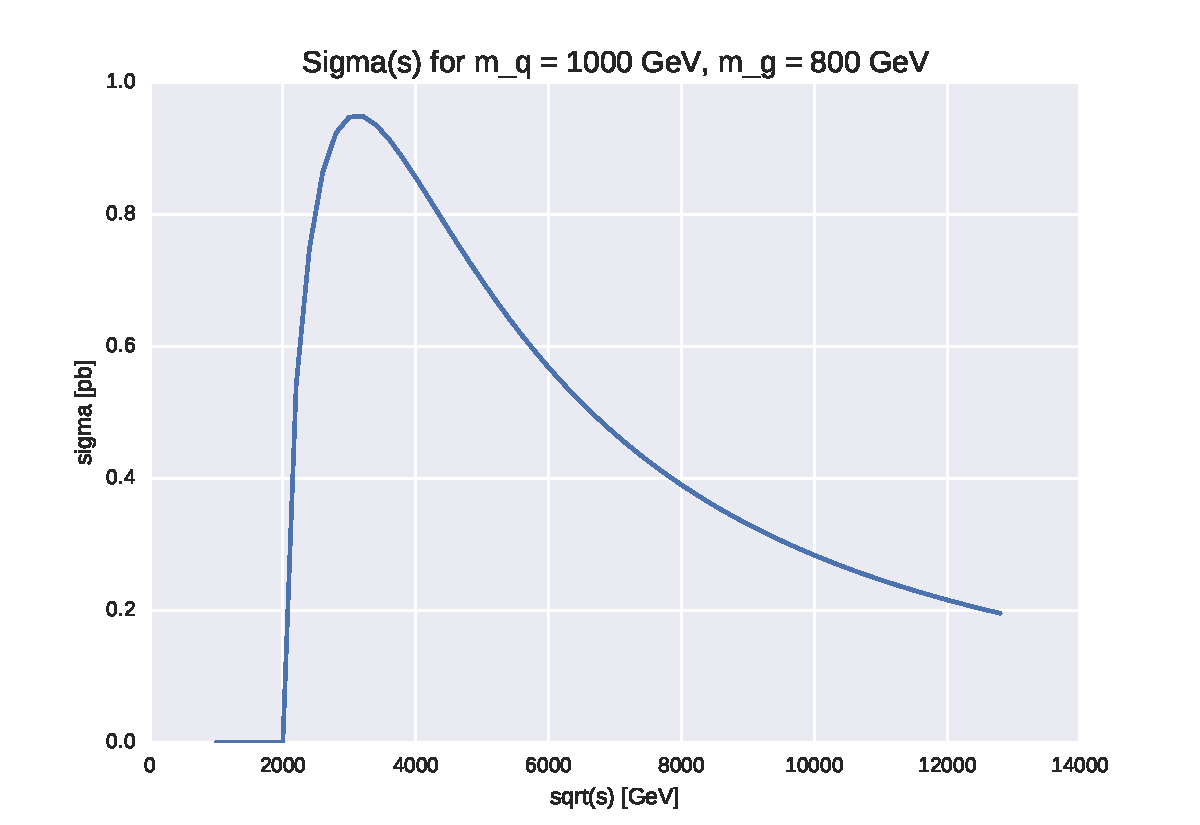
\includegraphics[scale=0.7]{plots/sigma_diff_test.pdf}
\caption{The cross section (before PDF) for squark production $qq \rightarrow \tilde{q} \tilde{q}$, where $m_{\tilde{q}}= 1000$ GeV and $m_{\tilde{g}}=800$ GeV.}
\label{fig:: sigma_diff 800 1000}
\end{figure}


\subsection*{Parton Distribution Function}
\begin{flushleft}
When we collide protons we are really interested in colliding their partons, the gluons and quarks. A proton consists of valence quarks -- its three main constituents $uud$ -- and a sea of virtual quarks and gluons. When these collide however, we don't know how much of the total momentum of the proton they have. Therefore, in order to find the total cross section it is necessary to use a convolution integral to integrate over the possible different fractions of total momentum $x_1$, $x_2$ the incoming quarks can have
\begin{align*}
\sigma_{total} &= \int f(x_1) f(x_2) \sigma(\hat{s}) dx_1 dx_2,
\end{align*}
where $\hat{s} = x_1 x_2 s$. The calculations are done using the following parameters
\begin{table}[H]
\centering
\begin{tabular}{|c|c|}
\hline
Parameter & Value\\
\hline
$m_{\tilde{q}}$ & $500-2000$ GeV\\
$m_{\tilde{g}}$ & $800-2000$ GeV\\
$Q^2$ & $m^2=m_{\tilde{q}}^2$\\
$\hat{\alpha}_s$ & 0.1148 \\
\hline
\end{tabular}
\end{table}
A Parton Distribution Function (PDF) like $f(x)$ is a probability distribution for the momentum fraction. They are not known a priori, and must be determined experimentally. The PDFs used in this project are generated by \textit{LHAPDF}, and an example for the PDFs of $\tilde{u}$ and $\tilde{d}$ are found in Fig. (\ref{fig::PDF 1 2}). This program takes $Q^2$ as an input, which is an energy scale for the renormalization of the theory.
\end{flushleft}

\begin{figure}[H]
\centering
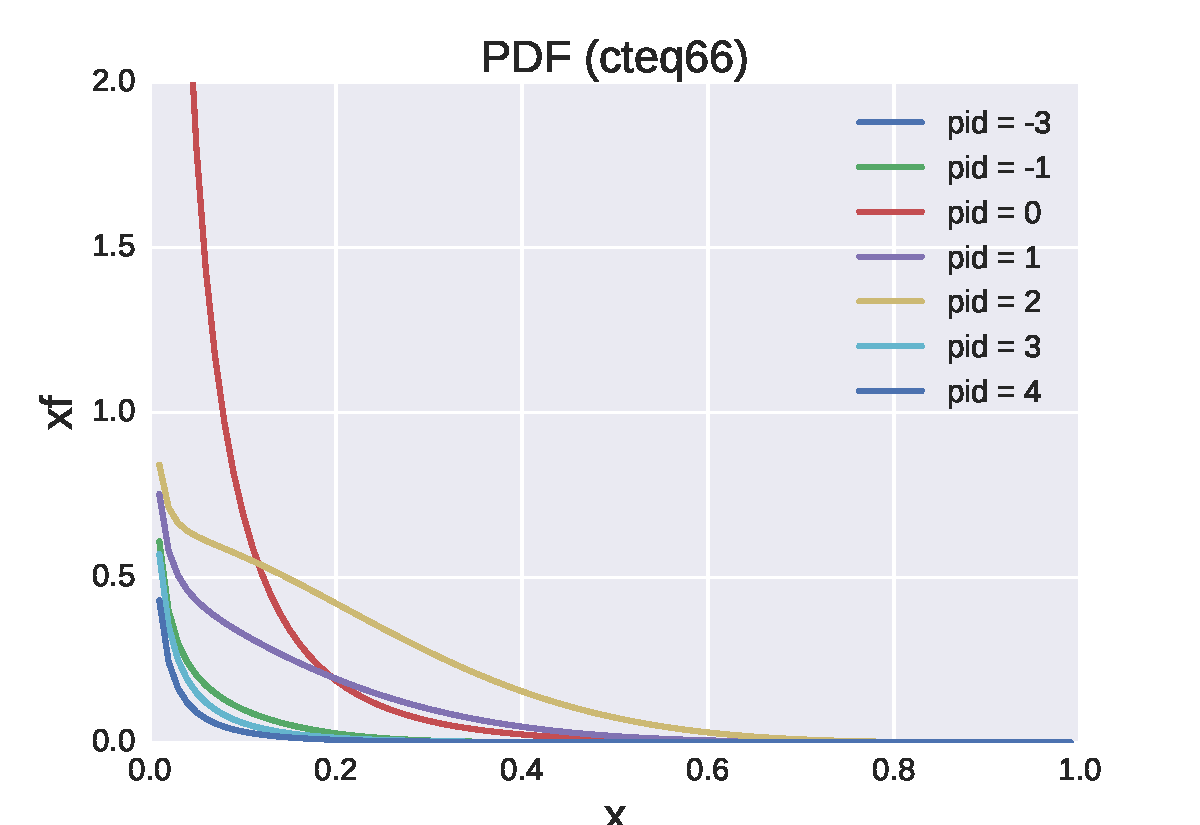
\includegraphics[scale=0.5]{plots/PDF_pids12.pdf}
\caption{Parton distribution function for several pid (quark numbers), generated by \textit{LHAPDF}, $Q=m_{\tilde{q}}$. Here, pid$0$=gluon, pid$1$=up etc.}
\label{fig::PDF 1 2}
\end{figure}



\section{Prospino}
\subsection*{Why NLO terms?}
\begin{flushleft}
Cross sections are really a perturbative expansion in a parameter called the coupling constant, which we can call $\lambda$. We can imagine the expansion as 
\begin{align*}
\sigma(\mathcal{A}, \mathcal{B} \rightarrow 1,2) = \lambda \sigma_1 + \lambda^2 \sigma_2 +...
\end{align*}
In electromagnetism, for example, the coupling constant is the electric charge $\lambda=e$.
Since $e$ is so small, we can to some extent only use the first order terms and get a pretty good prediction for a cross section. Including more terms, however, would reduce the error in the cross section. Calculating the NLO terms for $q q \rightarrow \tilde{q} \tilde{q}$ should therefore reduce the dependence on the renormalization scale considerably, thereby making the predictions less uncertain. Unfortunately, the tediousness and complexity of the calculation increases exponentially with the order of $e$. Luckily, many corrections can be calculated using programs such as Prospino \cite{beenakker1996prospino}. An example using $m_{\tilde{q}}=1000$ GeV and $m_{\tilde{g}}=800$ GeV is plotted in Fig. (\ref{fig:: prospino example}). The difference between leading order (LO) and next-to-leading (NLO) is also plotted, and shows that the NLO correction grows with the energy scale.

\end{flushleft}
\begin{figure}[H]
\centering
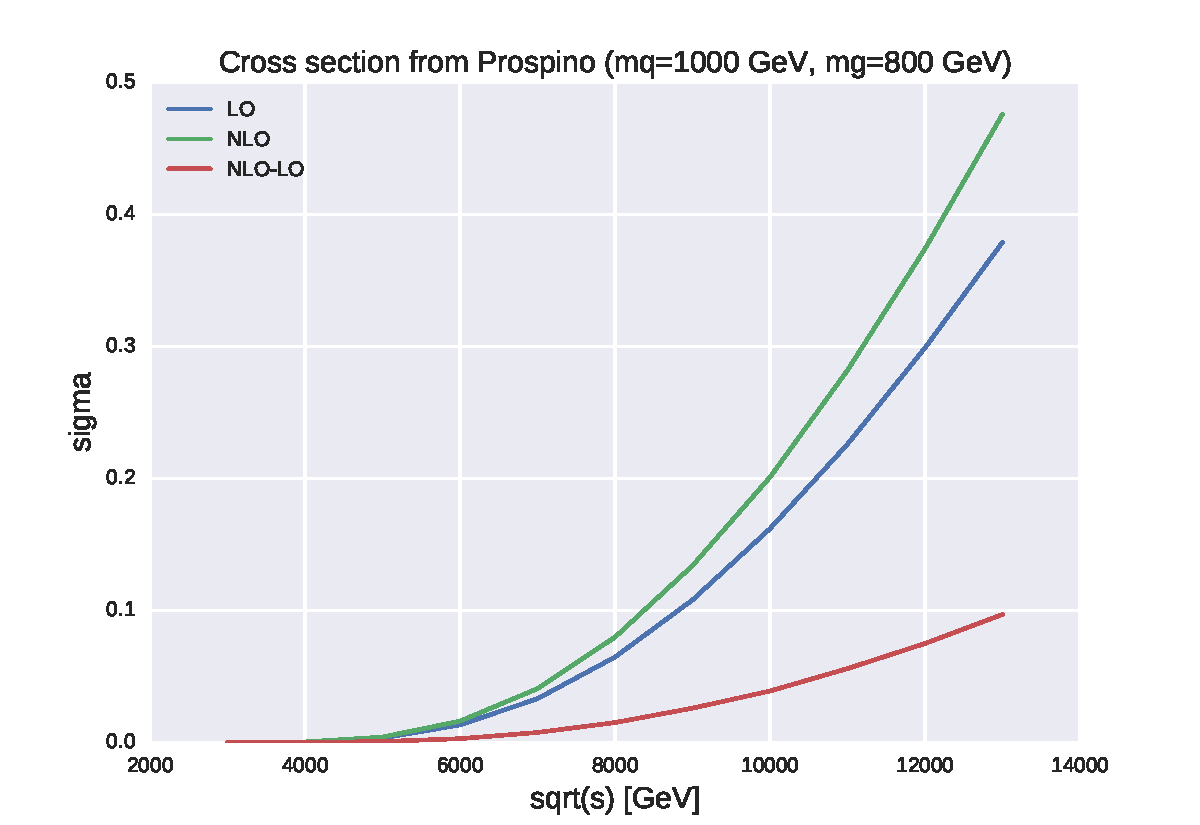
\includegraphics[scale=0.7]{prospino/prospino_800_1000.pdf}
\caption{Cross section for $qq \rightarrow \tilde{q} \tilde{q}$ calculated using Prospino \cite{beenakker1996prospino} both to leading order (LO) and next-to-leading order (NLO). The masses are $m_{\tilde{q}}=1000$ GeV and $m_{\tilde{q}}=800$ GeV, and $\Delta \sqrt{s}=1000$ GeV.}
\label{fig:: prospino example}
\end{figure}



\section{Experimental search for SUSY}
\begin{flushleft}
Squark production could be characterized by the production of jets and missing momentum, owing to the lightest supersymmetric particle $\chi_1^0$ (neutralino). If $R$-parity is conserved and the lightest sparticle (LSP) is stable and only weakly interacting it should escape detection, and lead to a large amout of missing energy. Since we will use data from the OpenATLAS Data, we will need to look for a signature that contains at least one lepton in the final state. A possible process is 
\begin{align*}
q_iq_j \rightarrow \tilde{q}_i \tilde{q}_j \rightarrow \tilde{\chi}_1^0 \tilde{\chi}_1^0 q_i q_j WW,
\end{align*}
for which the supersymmetric shower is shown in the Feynman diagram in Fig. (\ref{fig:: decay at ATLAS}). In the analysis we will have to consider the \textbf{missing transverse energy}, or transverse mass, \textbf{hadronic jets} and a \textbf{single lepton}. We will also have to take into account the \textbf{background signal}.
\begin{figure}[H]
\centering
\begin{tikzpicture}
\begin{feynman}
\vertex (p1) {\(p\)}; 
\vertex [below right=of p1, blob] (p) {}; 
\vertex [below left=of p] (p2){\(p\)}; 
%----------------------------------
\vertex [right=1.5cm of p] (mid1);\vertex [above=0.7cm of mid1] (s1);
\vertex [below =0.7cm of mid1] (s2);
\vertex [right=1.5cm of s1] (q1); 
\vertex [right=1.5cm of s2] (q2) ; 
%---------------------------------
\vertex [right=1cm of q1] (r1) ; %W
\vertex [right=1cm of q2] (r2) ; %W
%--------------------------------
\vertex [right=1cm of r1] (rl) {\(l\)};
\vertex [above=0.7cm of rl] (rn) {\(\nu\)};
\vertex [right=1cm of r2] (rq1) {\(q\)};
\vertex [below=0.7cm of rq1] (rq2) {\(q\)};
%--------------------------------
\vertex [above=0.7cm of rn, color=magenta] (r11) {\(\tilde{\chi}_1^0\)};
\vertex [below=0.7cm of rq2, color=magenta] (r22) {\(\tilde{\chi}_1^0\)};
\vertex [above=0.7cm of r11] (q11) {\(q\)}; 
\vertex [below=0.7cm of r22] (q22) {\(q\)};
\diagram{
(p1)--(p)--(p2), 
(p) --[scalar, edge label={\(\tilde{q}\)}, color=magenta] (s1), 
(s2) --[scalar, edge label={\(\tilde{q}\)}, color=magenta] (p); 
(q1) --[photon, plain, edge label= {\(\tilde{\chi}_1^{\pm}\)}, , color=magenta] (s1); 
(s1) -- (q11); (s2) --[photon, plain, edge label= {\(\tilde{\chi}_1^{\pm}\)}, color=magenta] (q2); 
(s2) -- (q22), 
(r1) -- [photon, edge label={\(W\)}] (q1),
 (q1) --[photon, plain, color=magenta](r11), 
 (q2) --[photon, edge label={\(W\)}] (r2), 
 (q2) --[photon, plain, color=magenta] (r22),
(rn)--(r1) -- (rl), 
(rq1) -- (r2) -- (rq2)
};
\end{feynman}
\end{tikzpicture}
\caption{Possible signature of a supersymmetric QCD process, with four quark jets, a lepton and large missing transverse energy in the final state.}
\label{fig:: decay at ATLAS}
\end{figure}
In the decay we are considering, the simplified model focuses on left-handed squarks which pair-produce strongly interacting sparticles, which then decay into a $W$ boson and the LSP. The free parameters are the squark and gluino masses, and either the chargino mass while the $\tilde{\chi}_1^0$ mass is fixed at $60$ Gev for $\sqrt{s}=8$ TeV, or the $\tilde{\chi}_1^0$ while $m_{\tilde{\chi}^{\pm}}=(m_{\tilde{g} / \tilde{q}}+ m_{\tilde{\chi}^0_1})/2$. The data recorded in the search of 2015 and 2016 in $\sqrt{s}=13$ proton-proton collisions at the LHC corresponds to an integrated luminosity of $36.1$ fb$^{-1}$, while we here use data at $8$ TeV with integrated luminosity $1$ fb$^{-1}$.
\end{flushleft}

\begin{flushleft}
Other possibilities are simplified models considering gluino-mediated production of top-squarks, and phenomenological models such as the super-gravity-mediated SUSY breaking (mSUGRA/CMSSM), bilinear R-parity violation (bRPV), natural gauge mediation (nGM) and a non-universal Higgs-boson mass wth gaugigo mediation (NUHMG) \cite{carquin2015search}.
\end{flushleft}

%\subsection*{Hadroproduction of jets}
%\begin{flushleft}
%High energy interactions of hadrons are described by the QCD improved parton model \cite{ellis2003qcd}. Since at high energies the protons behave like a sea of valence quarks and virtual gluons and quarks, a hard scattering process is essentially a collision between 'broad band' beams of partons. The partons, the quarks and gluons, possess different fractions of the total momenta of the incoming hadrons. For two colliding hadrons, we can write the cross section as 
%\begin{align*}
%\sigma (P_1, P_2) = \sum_{i,j} \int dx_1 dx_2 f_i(x_1, \mu^2) f_j(x_2, \mu^2) \hat{\sigma_{ij}} (p1, p2, \alpha_s(\mu^2), Q^2/\mu^2),
%\end{align*}
%where $P_1$ and $P_2$ are the momenta of the incoming hadrons, $p_1 = x_1P_1$ and $p_2 = x_2P_2$ are the momenta of the colliding partons, $\mu^2$ is the factorization scale and $f_i(x_k, \mu^2)$ are the Parton Distribution functions, which must be determined experimentally. $\hat{\sigma}_{ij}$ is the short distance cross section for partons $i$ and $j$. 
%\end{flushleft}

\subsection*{Kinematics}
\begin{flushleft}
Because of the spectrum of ingoing longitudinal momenta, the center of mass frame of final particles is often boosted with respect to the initial frame. We therefore introduce kinematic variables that are invariant, or transform simply, under Lorentz boosts in the $z$-direction (longitudinal direction). These parameters are the rapidity $y$, the pseudorapidity $\eta$, the transverse momentum $p_T$ and the azimuthal angle $\phi$. We can write the four-momentum of a particle in terms of these
\begin{align*}
p^{\mu} = (E, p_x, p_y, p_z) = (m_T \cosh y, p_T \sin \phi, p_T \cos \phi, m_T \sinh y),
\end{align*}
where $m_T$ is the transverse mass, defined as $m_T \equiv \sqrt{p_T^2 + m^2}$. The rapidity is useful because it is invariant under boosts along the longitudinal directoin, but the pseudo-rapidity is more commonly used as it involves the angle $\theta$ from the beam direction, which is experimentally measured. They are defined as
\begin{align*}
&y = \frac{1}{2} \ln \Big( \frac{E+p_z}{E-p_z} \Big); &
\eta = - \ln \tan \big( \frac{\theta}{2} \big).
\end{align*}
In addition, it is more common to use the transverse energy $E_T$ rather than the transverse momentum $p_T$, as this is what what is measured in a hadron calorimeter. It is given as
\begin{align*}
E_T = E \sin \theta.
\end{align*}
\end{flushleft}

\begin{flushleft}
To produce a gluino at the LHC for $\sqrt{s}=13$ TeV, would require a parton momentum fraction according to the relation
\begin{align*}
\braket{x} = \sqrt{\tau} = \frac{M}{\sqrt{s}},
\end{align*}
where $M= 2m_{\tilde{g}}$ for this process. Some values of $\braket{x}$ are shown in Tab. (\ref{tab:: momentum fractions x}).
\begin{table}[H]
\centering
\begin{tabular}{|c|c|}
\hline
$m_{\tilde{g}}$ [GeV] & $\braket{x}$\\
\hline
800 & 0.0615\\
1200 & 0.0923\\
1800 & 0.1385
\\
\hline
\end{tabular}
\caption{Momentum fraction $\braket{x}$ needed in order to produce a gluino of mass $m_{\tilde{g}}$ for the LHC running at $\sqrt{s}=13$ TeV.}
\label{tab:: momentum fractions x}
\end{table}
\end{flushleft}

\subsection*{Background}
\begin{flushleft}
The main background signals for this process come from top-quark production and $W+$jets. The signals from $t \bar{t}$ and $W$ are distinguished by a requirement on the number of $b$-tagged jets. $b$-tagging is reconstructing and filtering jets based on impact parameter and/or lifetime (B-mesons have a long lifetime because they decay weakly). Top quarks almost always decay to $Wb$ ($V_{tb}=0.99915 \pm 0.00005$). The $W \rightarrow tX$ decay is kinematically forbidden as $m_t > m_W$. However, a single top can be produced through a virtual $W$. The signature of $t \bar{t}$ can for example be 1 muon, 1 electron, 2 $b-$jets and 1 light jets, which is very similar to our signal. The typical decays of $t \bar{t}$ are (from the Particle Data Group)
\begin{align*}
t \bar{t} & \rightarrow W^+b W^- \bar{b} \rightarrow q \bar{q}_i b q_j \bar{q}_k \bar{b}, & (45.7\%) \\
t \bar{t} & \rightarrow W^+ b W^- \bar{b} \rightarrow q \bar{q}_i b \ell^- \bar{\nu}_{\ell} \bar{b} + \ell^+ \nu_{\ell} b q_j \bar{q}_k \bar{b}, &(43.8 \%)\\
t \bar{t} & \rightarrow W^+ b W^- \bar{b} \rightarrow \bar{\ell}_i \nu_{\ell} b \ell_j \bar{\nu}_{\ell_j} \bar{b}. &(10.5 \%)
\end{align*}
\end{flushleft}
\begin{figure}[H]
\begin{tikzpicture}
\begin{feynman}

\vertex (f1) {\(g\)}; \vertex [below right = of f1] (f); \vertex [below left= of f] (f2) {\(g\)}; \vertex [right = of f] (g); \vertex [above right=of g] (g1) {\(\bar{b}\)}; \vertex [below right= of g] (g2) {\(t\)}; 

\diagram{
(f2) --[fermion] (f) --[fermion] (f1); (f) --[photon, edge label={\(W\)}] (g); (g1) --[fermion] (g) --[fermion] (g2)
}; 

\hspace*{4.2cm};

\vertex (p1) {\(g\)}; \vertex [below right = of p1] (p); \vertex [below left= of p] (p2) {\(g\)}; \vertex [right = of p] (s); \vertex [above right=of s] (s1) {\(\bar{t}\)}; \vertex [below right= of s] (s2) {\(t\)}; 

\diagram{
(p2) --[gluon] (p) --[gluon] (p1); (p) --[gluon, edge label={\(g\)}] (s); (s1) --[fermion] (s) --[fermion] (s2)
}; 

\hspace*{4.2cm};

\vertex (q1) {\(\bar{q}\)}; \vertex [below right = of q1] (q); \vertex [below left= of p] (q2) {\(q\)}; \vertex [right = of q] (r); \vertex [above right=of r] (r1) {\(\bar{t}\)}; \vertex [below right= of r] (r2) {\(t\)}; 

\diagram{
(q2) --[fermion] (q) --[fermion] (q1); (q) --[gluon, edge label={\(g\)}] (r); (r1) --[fermion] (r) --[fermion] (r2)
}; 

\hspace*{4.2cm};

\vertex (m1) {\(\bar{q}\)}; \vertex [below right = of m1] (m); \vertex [below left= of m] (m2) {\(q\)}; \vertex [right = of m] (n); \vertex [above right=of n] (n1) {\(\ell, q\)}; \vertex [below right= of n] (n2) {\(\nu, \bar{q}'\)}; 

\diagram{
(m2) --[fermion] (m) --[fermion] (m1); (m) --[photon, edge label={\(W\)}] (n); (n1) --[fermion] (n) --[fermion] (n2)
}; 
\end{feynman}
\end{tikzpicture}
\caption{Background signals from $t \bar{t}$ and $W$. Top is produced through the strong force.}
\end{figure}

\subsection*{The ATLAS detector}
\begin{flushleft}
ATLAS is a multi-purpose detector which provides a nearly full solid angle coverage around the interaction point \cite{carquin2015search}. It consists of a tracking system surrounded by a thin superconducting solenoid providing a 2 T magnetic field, electromagnetic and hadronic calorimeters and muon spectrometer (MS).The ATLAS trigger system consists of three levels; the first level is a hardware-based system, while the second and third levels are software-based systems and are collectively referred to as the High Level Trigger (HLT) \cite{carquin2015search}.
\end{flushleft}


\section*{Analysis}
\begin{flushleft}
We will look for hard single-lepton signal regions, since the lepton ($e^{\pm}$ or $\mu^{\pm}$) comes from decay of $W^{\pm}$ and will therefore be very energetic (hard single lepton). This signal region is designed with lower jet multiplicities to cover squark production. The variables used in various cuts are the following. The transverse mass $m_T$ of the lepton $\ell$ and $\textbf{p}_T^{miss}$ is defined as
\begin{align*}
m_T = \sqrt{m^2 + p_x^2 + p_y^2}= \sqrt{2p_T^{\ell}E_T^{miss}(1- \cos [\Delta \phi(\vec{\ell}, \textbf{p}^{miss}_T)])}.
\end{align*}
The transverse mass is used to reject events containing a $W \rightarrow \ell \nu$. The inclusive effective mass, which is the sum of transverse momenta of the jets and leptons, and the missing energy, is defined as
\begin{align*}
m_{eff}^{inc} = \sum_{i=1}^{N_{\ell}} p^{\ell}_{T,i} + \sum^{N_{jet}}_{j=1} p_{T,j} + E_T^{miss}.
\end{align*}
The inclusive effective mass provides a good discrimination against the SM background without being sensitive to the details of the SUSY cascades. We also define an exclusive effective mass, which is similar to $m_{eff}^{inc}$, except that it only sums over the three leading signal jets. The ratio $E_T^{miss}/m_{eff}^{excl}$ is used to remove events with large $E_T^{miss}$ that simply come from a poorly constructed jet. In addition, a veto is placed on the presence of a second lepton. The cuts can be found in Tab. (\ref{tab::signal cuts}).
\end{flushleft}
\begin{table}[H]
\centering
\begin{tabular}{c}
\textbf{Hard single lepton (3-jet)}
\end{tabular}

\begin{tabular}{|l|c|}
\hline
$N_{\ell}$ & 1 electron or muon\\
\hline
$p_T^{\ell}$[GeV] & $> 25$\\
\hline
Lepton veto & $p_T^{2^{nd} \text{ lepton}}< 10$ GeV\\
\hline
$N_{jet}$ & $\geq 3$\\
\hline
$p_T^{jet}$ [GeV] & $>80, 80, 30$\\
\hline
Jet veto & ($p_T^{5^{th} \text{ jet}} < 40$ GeV)\\
\hline
$E_T^{miss}$ [GeV] & $>500$\\
\hline 
$m_T$ [GeV] & $> 150$\\
\hline
$E_T^{miss}/m_{eff}^{excl}$ & $>0.3$\\
\hline 
$m_{eff}^{incl}$ [GeV] & $>1400$\\
\hline
\end{tabular} 
\caption{Cuts for analysis. The rows $N_{\ell}$-$N_{jet}$ are specific for the specific process, and so are implemented from the start, while the others are introduced one by one.}
\label{tab::signal cuts}
\end{table}


\section*{Results}

\subsection*{Calculating the LO cross section}

\begin{flushleft}
As can be seen from Fig. (\ref{fig:: results LO varying mg mq}), the leading order (LO) term of the cross section is higher for a lower squark and gluino mass, reaching a maximum at $m_{\tilde{g}} = m_{\tilde{q}}=800$ GeV for high energies. For $m_{\tilde{g}}=2000$ GeV the cross section at high energies is maximized for $m_{\tilde{q}}=1000$ GeV. However, as the gluino mass increases, the low squark mass begins to give a negative contribution to the cross section. To find the reason for this unphysical value, $\sigma$ before PDF-integration was plotted for $m_{\tilde{q}}=800$ GeV and $m_{\tilde{q}}=2000$ GeV (Fig. (\ref{fig:: 800 2000 med og uten pdf})), and LO and NLO were also plotted using Prospino (Fig. (\ref{fig:: sigma 2000-800 LO og NLO})). None of these have negative values. The PDFs are not negative, as can be seen from Fig. (\ref{fig::PDF 1 2}). It is therefore likely that the negative cross sections in Fig. (\ref{fig:: results LO varying mg mq}) come from a numerical instability. More plots from this analysis can be found in the Github directory.
\end{flushleft}

\begin{figure}[H]
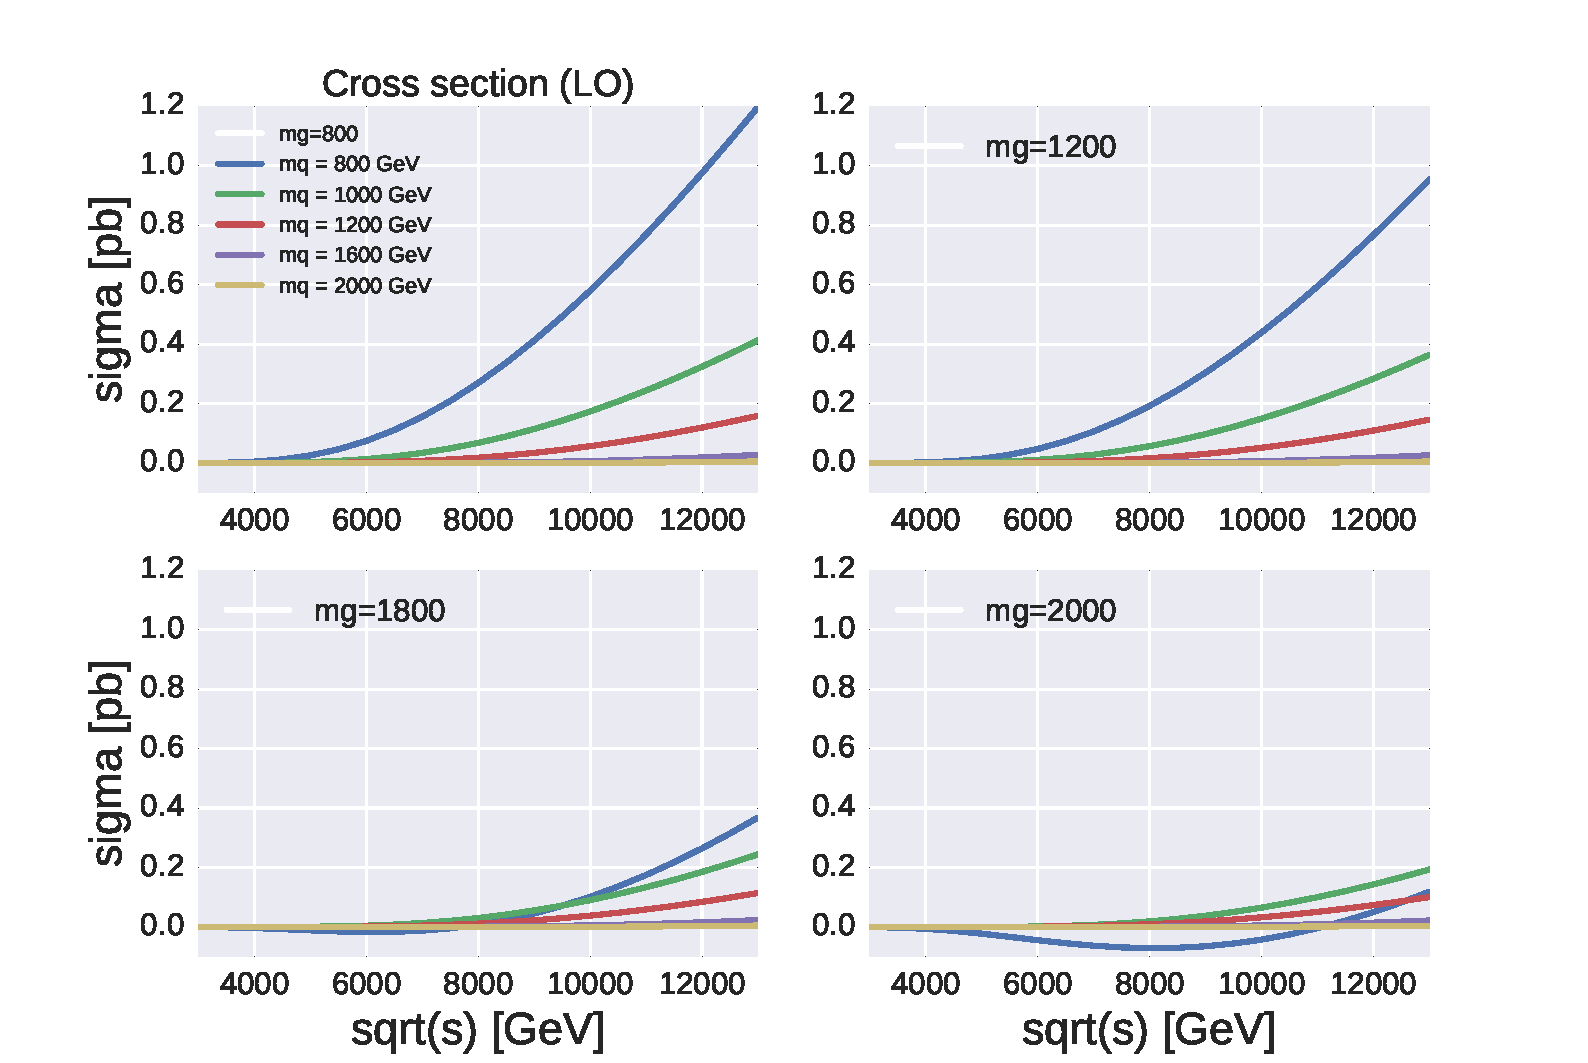
\includegraphics[scale=0.8]{plots/cropped_sigma_varymg_all.pdf}
\caption{Leading order contribution to cross section for $q_iq_j \rightarrow \tilde{q}_i \tilde{q}_j$, summed over quark flavors $u,d,c,s$ (equal and different incoming quarks). Integrated over PDF from cteq66, with a trapeze integral method using $N=1000$ integration steps. Gluino mass is $m_{\tilde{g}}=800$ GeV (upper left corner), $m_{\tilde{g}}=1200$ GeV (upper right corner), $m_{\tilde{g}}=1800$ GeV (lower left corner) and $m_{\tilde{g}}=2000$ GeV (lower right corner).}
\label{fig:: results LO varying mg mq}
\end{figure}

\begin{figure}[H]
\centering

\begin{minipage}{.5\textwidth}
  \centering
  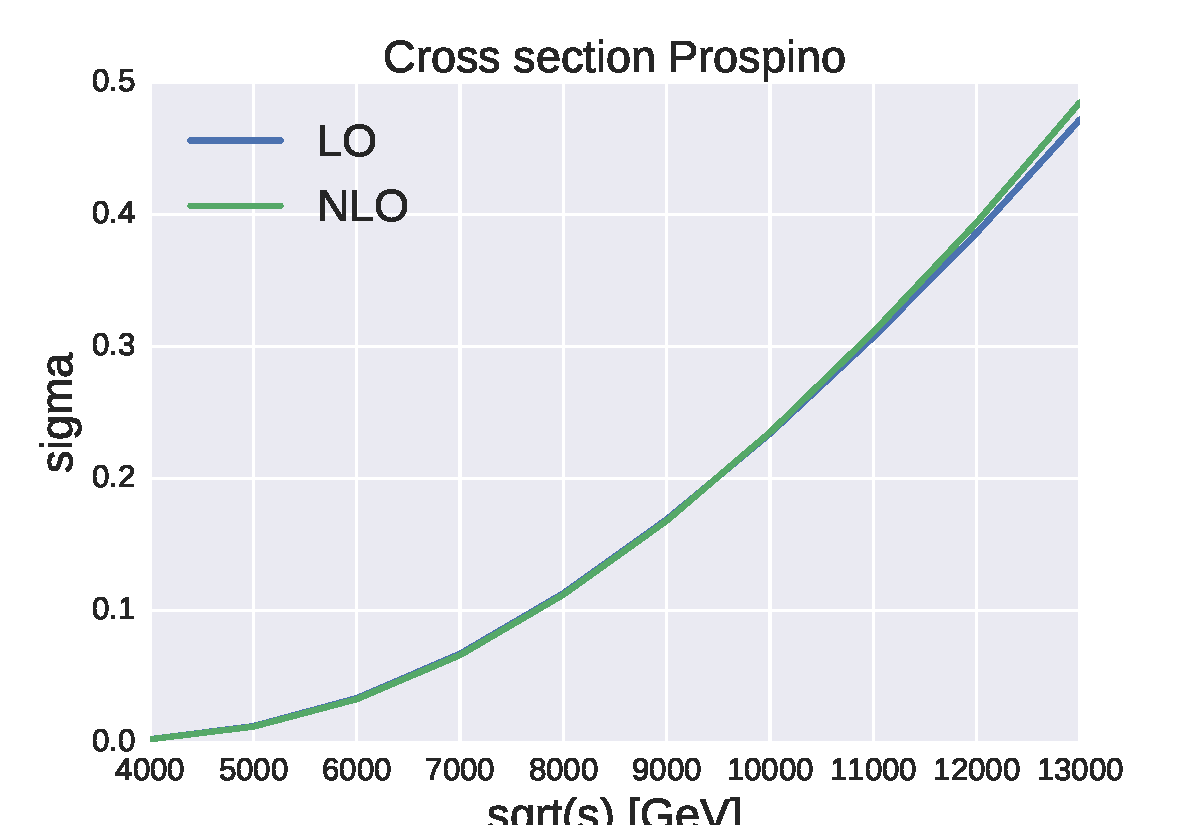
\includegraphics[width=1.1\linewidth]{plots/prospino_2000_800_tester.pdf}
\end{minipage}%
\begin{minipage}{.5\textwidth}
  \centering
  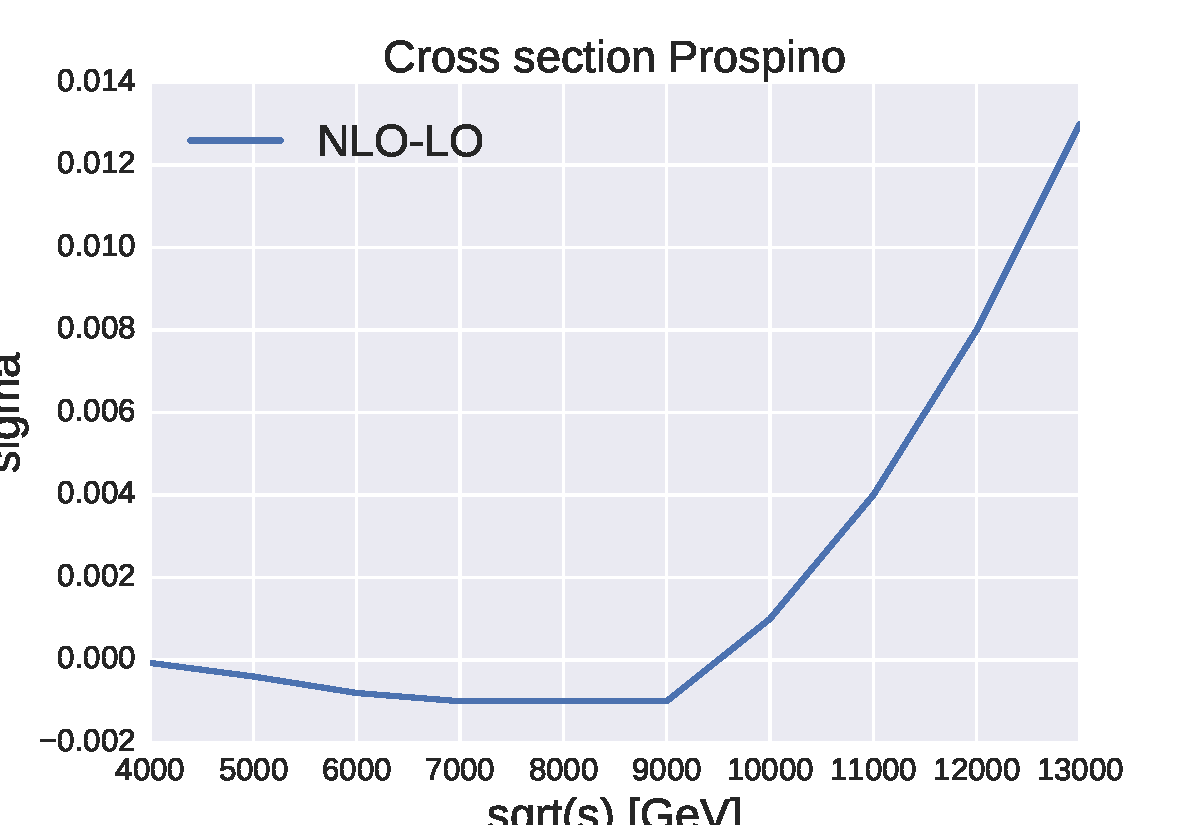
\includegraphics[width=1.1\linewidth]{plots/prospino_2000_800_tester_diff.pdf}
\end{minipage}

\caption{Cross section calculated using Prospino, for $m_{\tilde{g}}=2000$ GeV and $m_{\tilde{q}}=800$ GeV, for center of mass energies $\sqrt{s}=4000-13000$ GeV ($\Delta \sqrt{s}=1000$ GeV). Calculated both to leading order (LO) and next-to-leading order (NLO).}
\label{fig:: sigma 2000-800 LO og NLO}
\end{figure}

\begin{figure}[H]
\centering
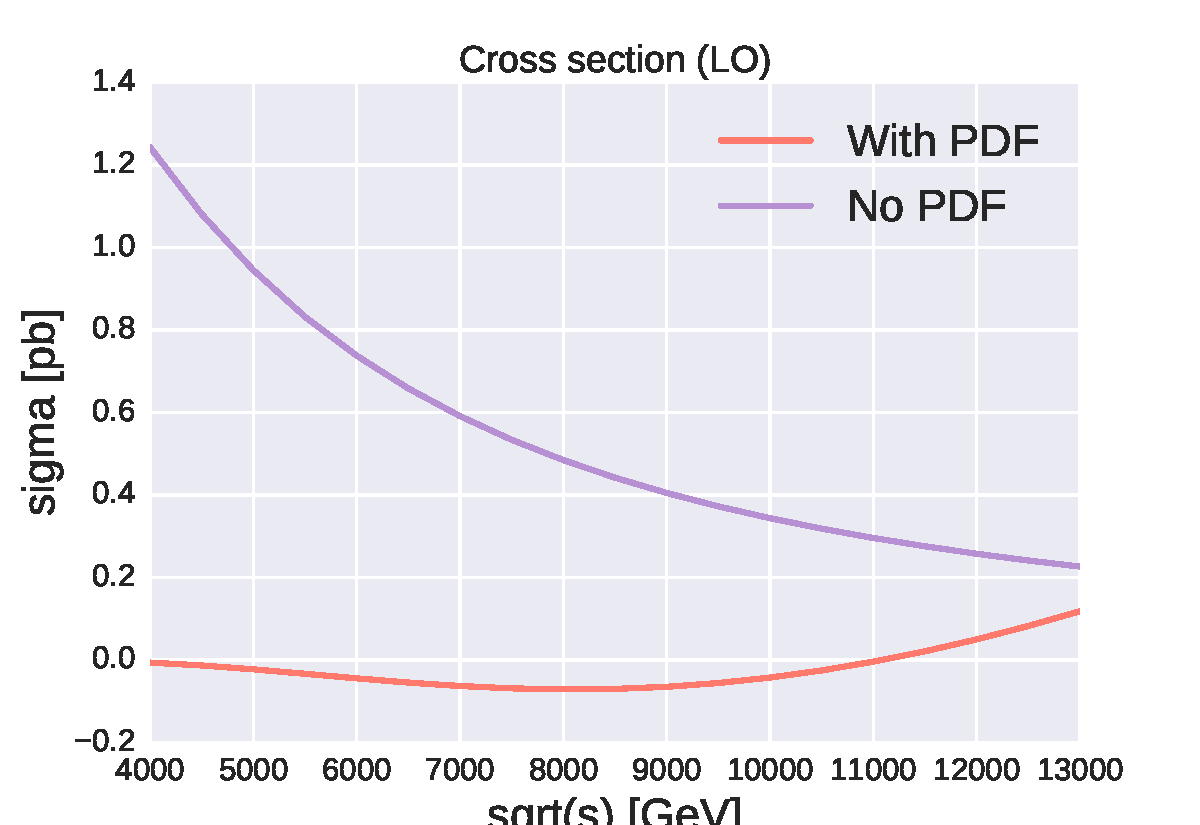
\includegraphics[scale=0.6]{plots/Negative_values_analysis/sigma_2000_800_pdftest.pdf}
\caption{Cross section calculated using analytically calculated $\sigma^B$. Plotted both pure $\sigma^B$ and after convolution integral with PDFs.}
\label{fig:: 800 2000 med og uten pdf}
\end{figure}

%\begin{figure}[H]
%\centering
%\includegraphics[scale=0.6]{plots/%Negative_values_analysis/%sigma_2000_800_anti.pdf}
%\caption{Cross section for $qq \rightarrow %\tilde{q}\tilde{q}$ using analytic calculation to LO. Convolution integral done summing over only quarks ('Quarks') and both quarks and antiquarks ('Quarks + antiquarks').}
%\label{fig:: included antiquarks}
%\end{figure}

%\begin{flushleft}
%As can be seen from Fig. (\ref{fig:: included antiquarks}), including the PDFs of the antiquarks removes much of the negative contribution. However, the cross section for $13$ TeV is now much larger ($\sim 1.2$ pb) than the one calculated using Prospino ($\sim 0.49$ pb).
%\end{flushleft}

\subsection*{Prospino}

\begin{flushleft}
The calculation from Prospino fits quite well with the analytic calculation, with the NLO term giving a positive correction. The cross sections from the analytic calculation, and from Prospino for LO and NLO at the masses $m_{\tilde{q}}=1000$ GeV and $m_{\tilde{g}}=800$ GeV are given in Fig. (\ref{fig:: prospino analytic comparison 800 1000}). The analytic cross section is somewhat higher than the LO from Prospino, but this could be from the choice of LHAPDF function or a numerical inaccuracy.
\end{flushleft}
\begin{figure}[H]
\centering
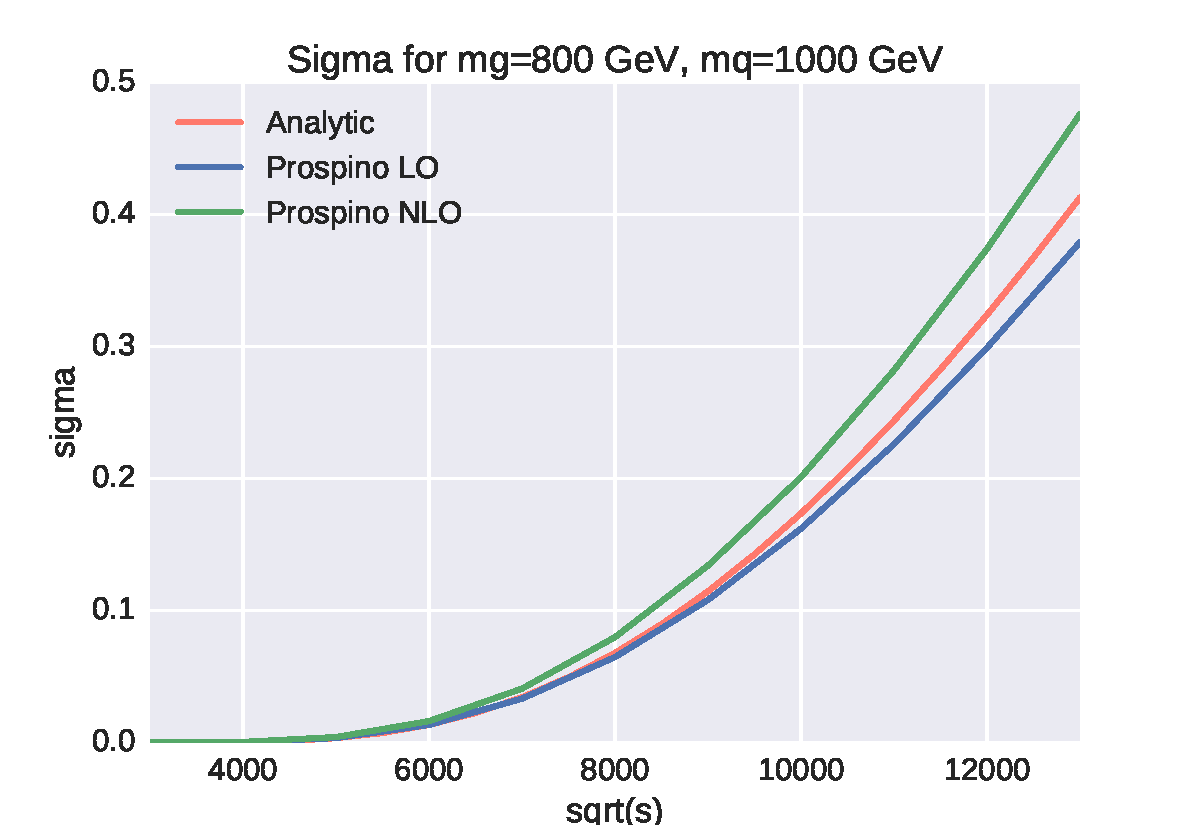
\includegraphics[scale=0.6]{plots/prospino_compare.pdf}
\caption{Cross section from analytic calculation, and Prospino LO and NLO contribution for $m_{\tilde{g}}=800$ GeV and $m_{\tilde{q}}=1000$ GeV.}
\label{fig:: prospino analytic comparison 800 1000}
\end{figure}

\subsection*{Analysis}

\begin{flushleft}
The analysis used three Monte Carlo samples, with different $m_{\tilde{q}}$, $m_{\tilde{\chi}_1^{\pm}}$ and $m_{\tilde{\chi}_1^0}$, and a very large gluino mass (around $3$ TeV) to rule out unwanted channels. The signal masses can be found in Tab. (\ref{tab:: signal masses}), along with their color in the histogram plots.
\end{flushleft}
\begin{table}[H]
\centering
\begin{tabular}{|l|c|c|c|c|}
\hline
Analysis name & $m_{\tilde{q}}$ [GeV] & $m_{\tilde{\chi}_1^{\pm}}$ [GeV] & $m_{\tilde{\chi}_1^0}$ [GeV] & Color\\
\hline
$SM_-SS_-onestepCC_-500_-260_-60$ &$500$ & $260$ & $60$ & Magenta\\ 
$SM_-SS_-onestepCC_-900_-260_-60$ &$900$ & $260$ & $60$ & Light pink\\ 
$SM_-SS_-onestepCC_-1100_-260_-60$ &$1100$ & $260$ & $60$ & Dark purple\\ 
\hline
\end{tabular}
\caption{Masses used in Monte Carlo simulations for analysis. Three different signals with different $m_{\tilde{q}}$.}
\label{tab:: signal masses}
\end{table}

\begin{flushleft}
A cross section plot is not done for $m_{\tilde{q}}=500$ GeV as squark masses under $800$ GeV have, for all intensive purposes, been excluded. $m_{\tilde{q}}=900,1100$ however, can be seen in Fig. (\ref{fig:: results LO varying mg mq}) (as somewhere between $800-100$ and $1000-1200$). The cross section is quite small, and decreasing for increasing $m_{\tilde{q}}$. Taking into account that we are considering large $m_{\tilde{g}}$, the bottom right plot ($m_{\tilde{g}}=2000$ GeV) is the most relevant. We see that the cross section here becomes very low. We therefore expect the signal from $m_{\tilde{q}}=1100$ GeV to be considerably lower than for $m_{\tilde{q}}=500$ GeV. 
\end{flushleft}

\begin{flushleft}
Histograms for the transverse mass and missing transverse energy are shown in Fig. (\ref{fig:: standard cuts hist}) for the standard cuts ($1-4$) in Tab. (\ref{tab::signal cuts}). In Fig. (\ref{fig:: etmiss hist}) The missing transverse energy in plotted with standard cuts to the left, and additional cuts (not $m_{eff}^{incl}$ or $E_T^{miss}/m_{eff}^{excl}$) to the right. The blue arrows indicate the cut on $E_T^{miss}$. In Fig. (\ref{fig:: mt hist}) the transverse mass is plotted for the same cuts. The signal for $m_{\tilde{q}}=500$ and $900$ GeV are somewhat improved with the cuts, while the $m_{\tilde{q}}=1100$ GeV signal dissappears almost completely. There is no significant excess of signal over background.
\end{flushleft}

\begin{flushleft}
The different cuts give new Z-scores, or standard deviations. The Z-score of a statistical distribution tells ut whether we can discard the null hypothesis on not. A Z-score of $1.67$ means we can make exclusions. Z-scores were calculated using ROOTs BinomialExpZ for the histograms after the transverse mass cut $m_T>150$, and again after the additional cuts of $E_T^{miss}/m_{eff}^{excl} > 0.3$ and $m_{eff}^{incl}> 1400$ GeV. With the luminosity of the data from ATLAS OpenData, which is $1$ fb$^{-1}$, the z-values are too low to exclude anything, see Tab. (\ref{tab:: z 1fb}). In Tab. (\ref{tab:: z 20fb}) the number of events has been multiplied by 20 to approximate the values from \cite{carquin2015search}, where $m_{\tilde{q}}=500$ GeV has been excluded. We then see that $z=2.0596$, so we can exclude this mass for this simplified model. Since the additional cuts seem to lower the Z-scores for luminosity $1$ fb$^{-1}$, they are not included in the plots in Fig. (\ref{fig:: etmiss hist})-(\ref{fig:: mt hist}). For luminosity $20$ fb$^{-1}$, however, the Z-score is increased with the cuts.
\end{flushleft}
\begin{table}[H]
\centering
\begin{tabular}{|c|c|c|}
\hline
$m_{\tilde{q}}$ [GeV] & Z before cuts & Z after cuts\\
\hline
$500$ & 0.6818 & 0.5985\\
$900$ & 0.1480 & 0.1065\\
$1100$ & Not enough events & Not enough events\\
\hline
\end{tabular}
\caption{Luminosity $1$ fb$^{-1}$.}
\label{tab:: z 1fb}
\end{table}

\begin{table}[H]
\centering
\begin{tabular}{|c|c|c|}
\hline
$m_{\tilde{q}}$ [GeV] & Z before cuts & Z after cuts\\
\hline
$500$ & 2.0596 & 2.2317\\
$900$ & 0.6583 & 0.7412\\
$1100$ & Not enough events & Not enough events\\
\hline
\end{tabular}
\caption{Luminosity $20$ fb$^{-1}$, so number of events was multiplied by 20.}
\label{tab:: z 20fb}
\end{table}


\begin{figure}[H]
\centering

\begin{minipage}{.5\textwidth}
  \centering
  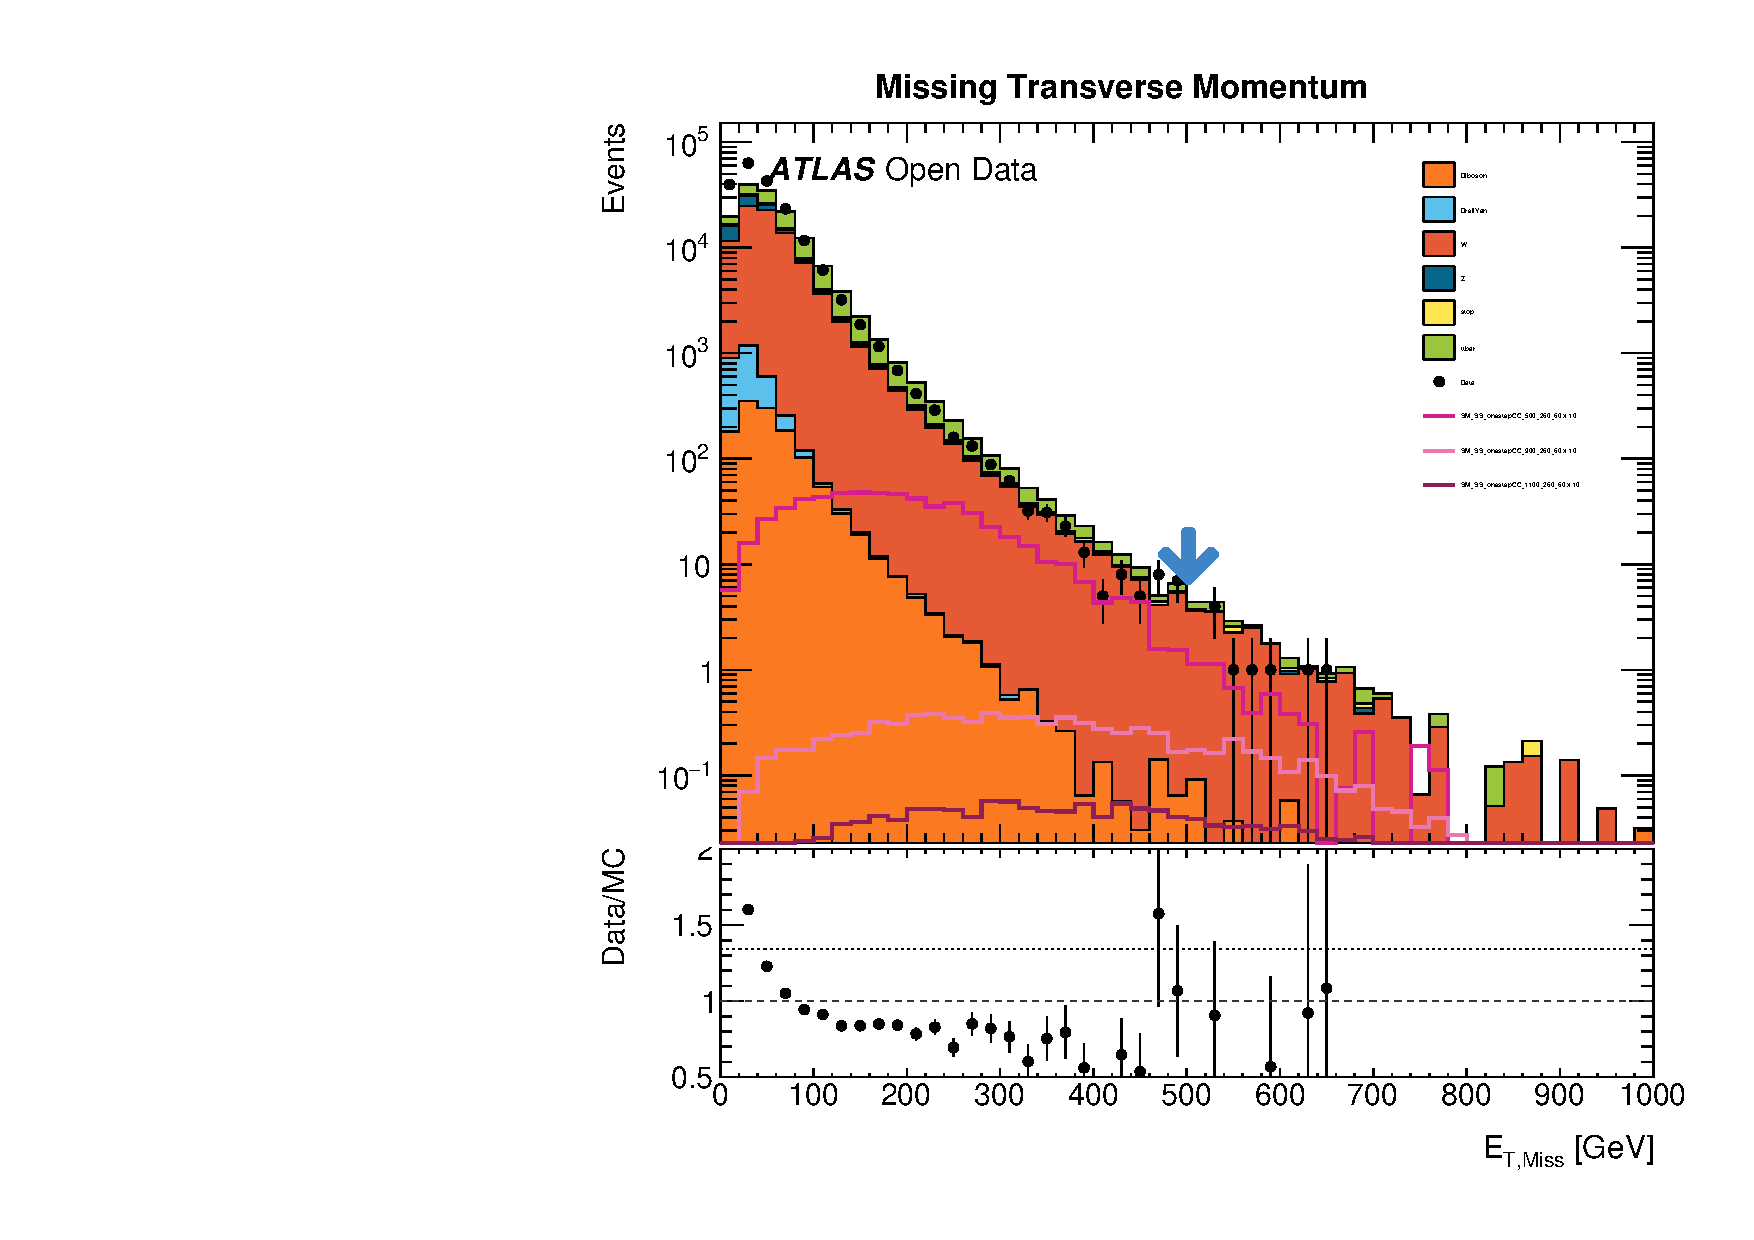
\includegraphics[width=1.\linewidth]{plots/Standard_Cut/cropped_etmiss_edited.pdf}
\end{minipage}%
\begin{minipage}{.5\textwidth}
  \centering
  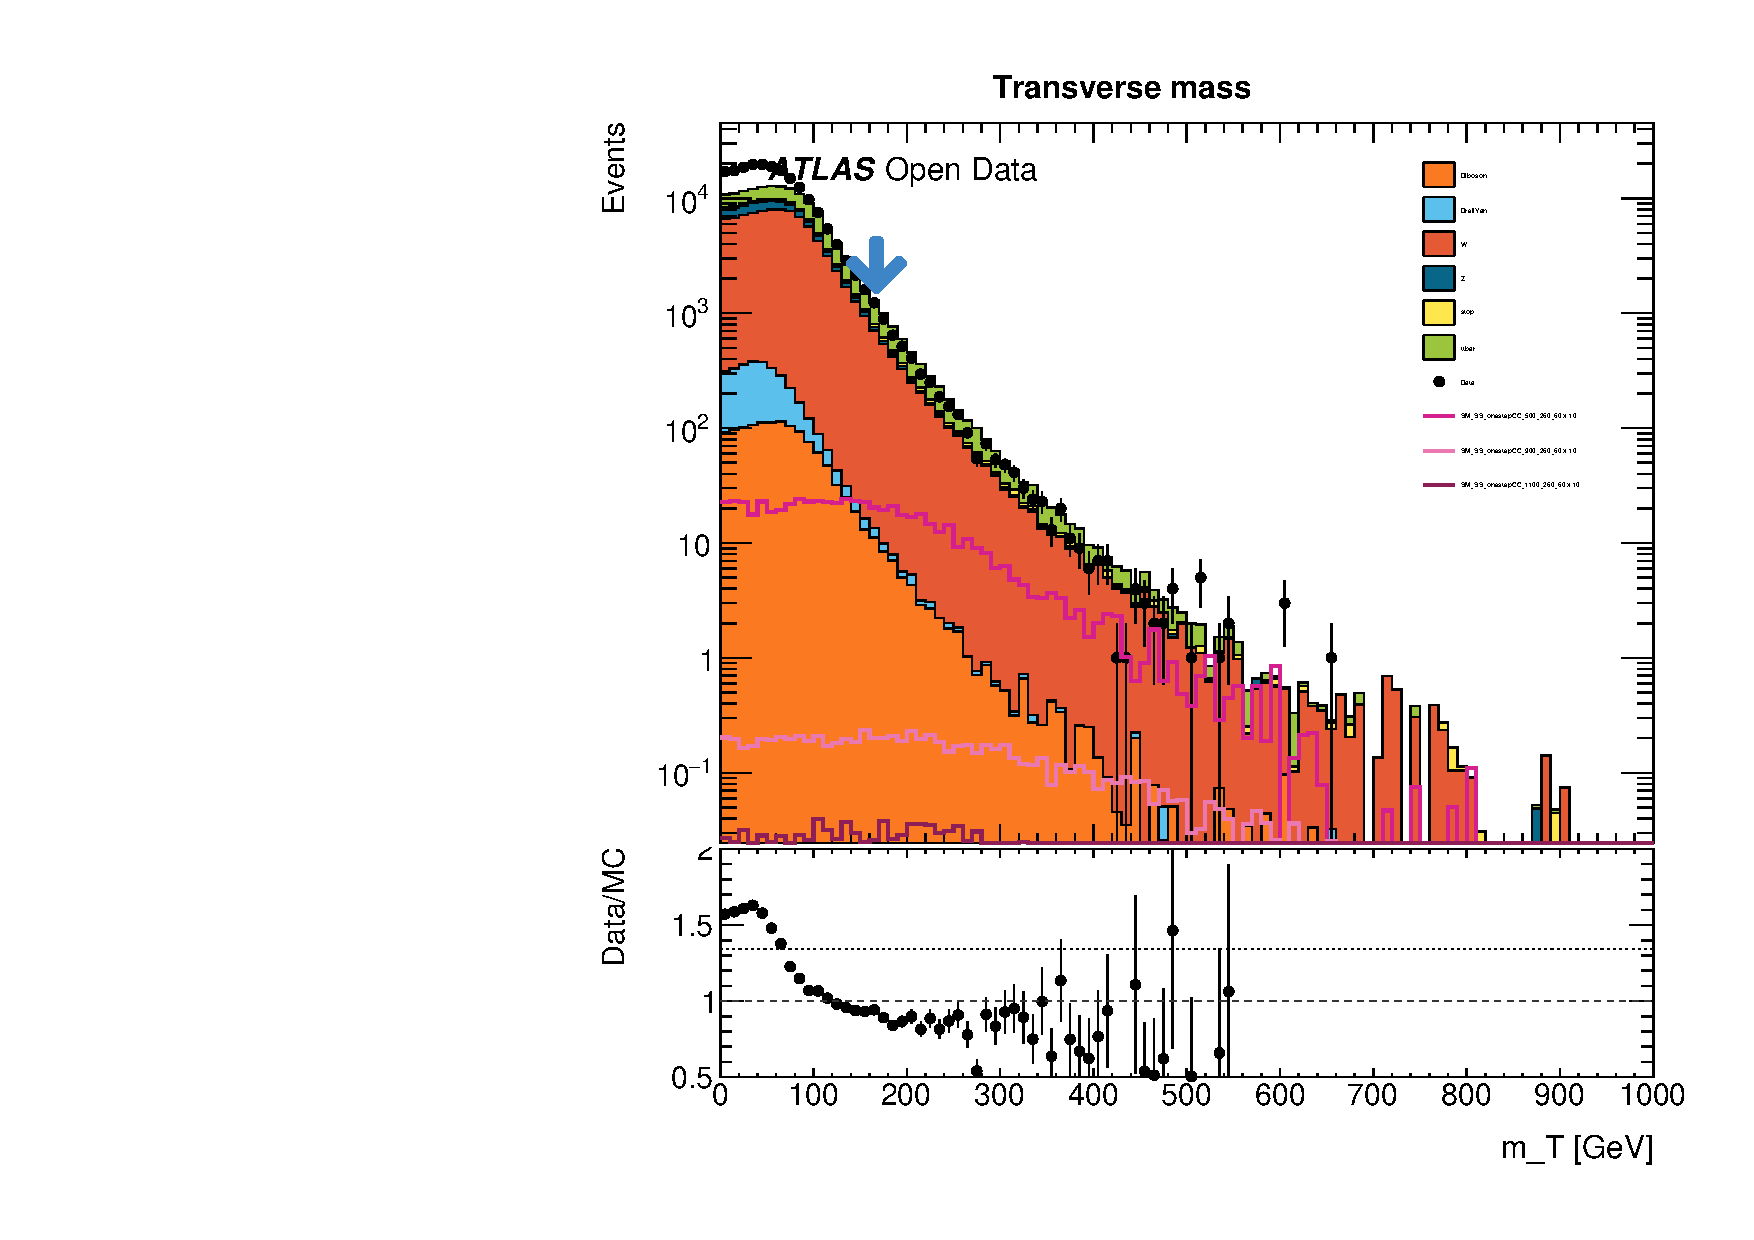
\includegraphics[width=1.\linewidth]{plots/Standard_Cut/cropped_mt_edited.pdf}
\end{minipage}

\caption{Histograms from simulation with standard cuts. The arrows indicate the cuts that will be made for $E_{T \text{ miss}} = 500$ GeV and $m_T = 150$ GeV.}
\label{fig:: standard cuts hist}
\end{figure}



\begin{figure}[H]
\centering

\begin{minipage}{.5\textwidth}
  \centering
  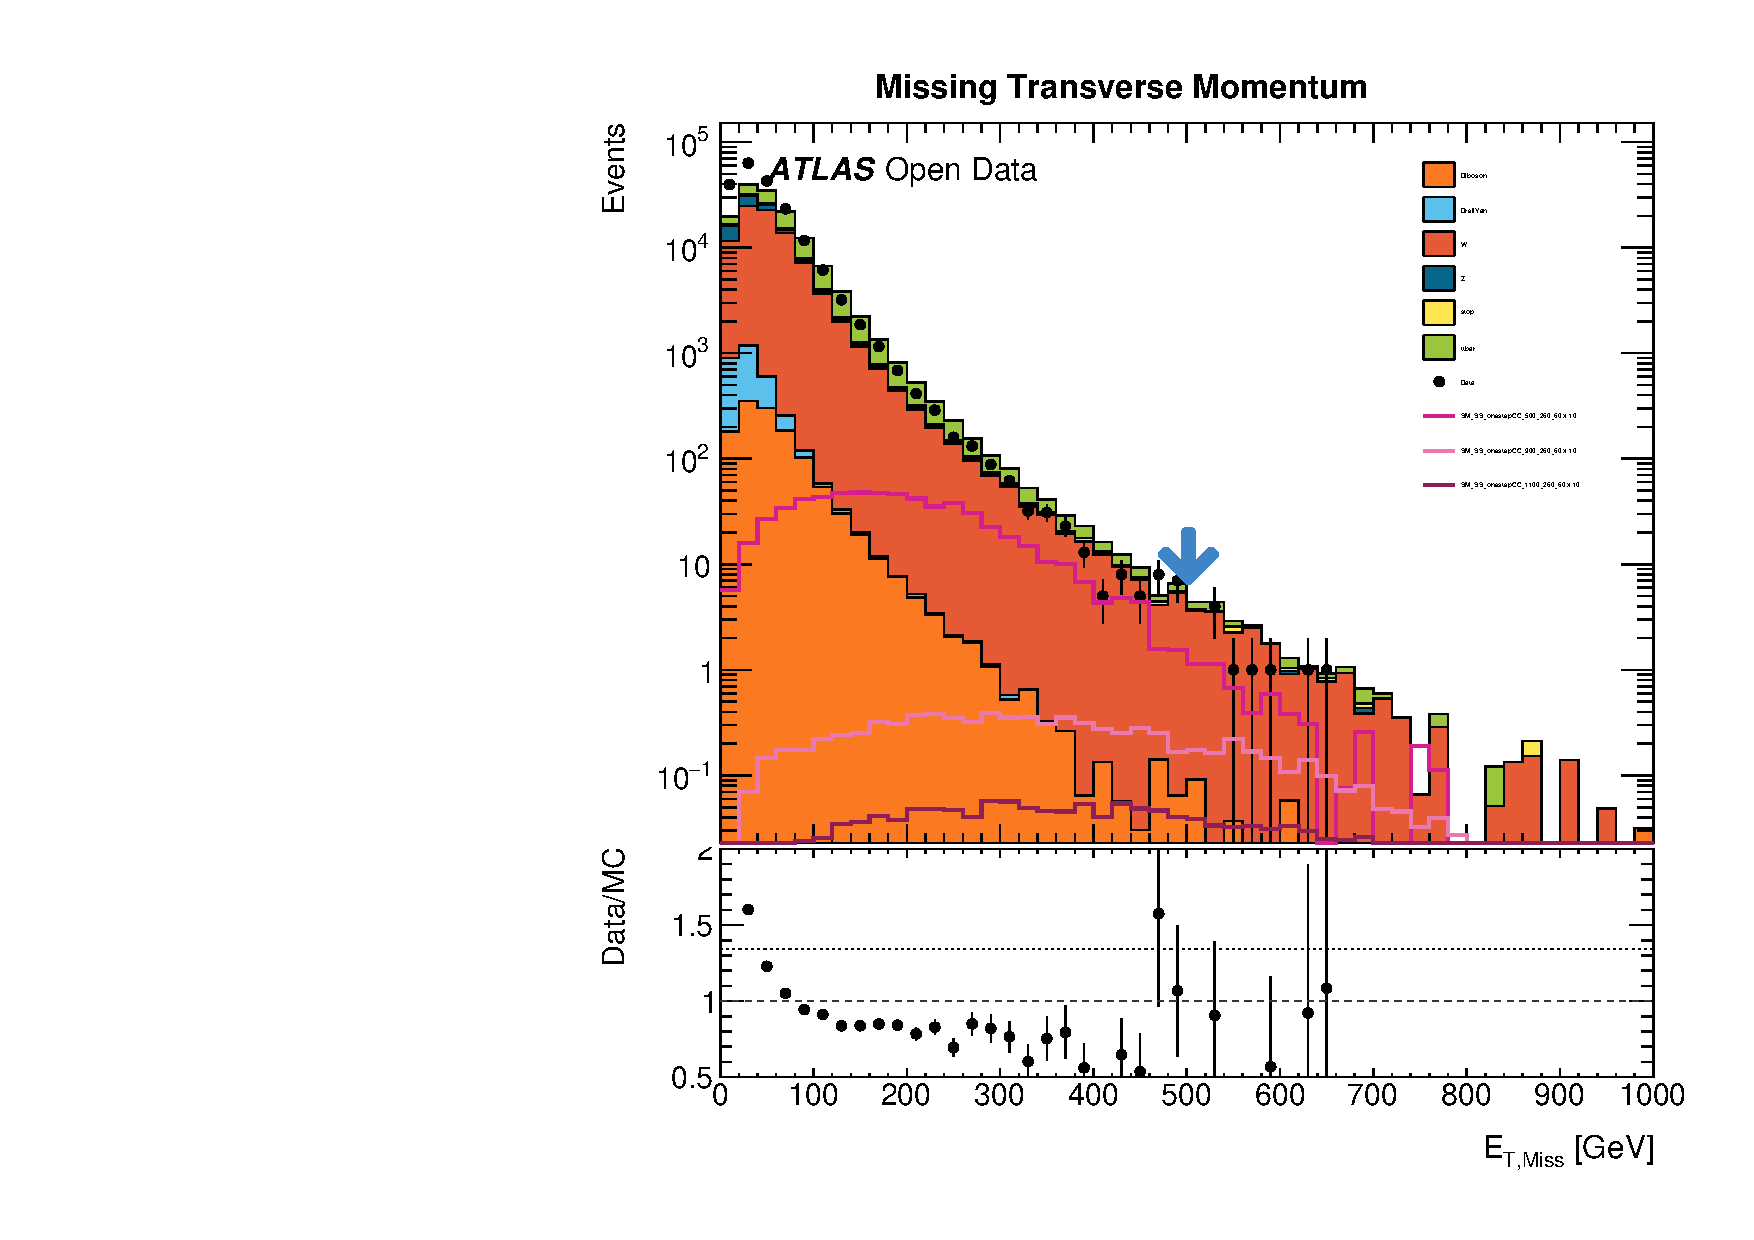
\includegraphics[width=1.\linewidth]{plots/Standard_Cut/cropped_etmiss_edited.pdf}
\end{minipage}%
\begin{minipage}{.5\textwidth}
  \centering
  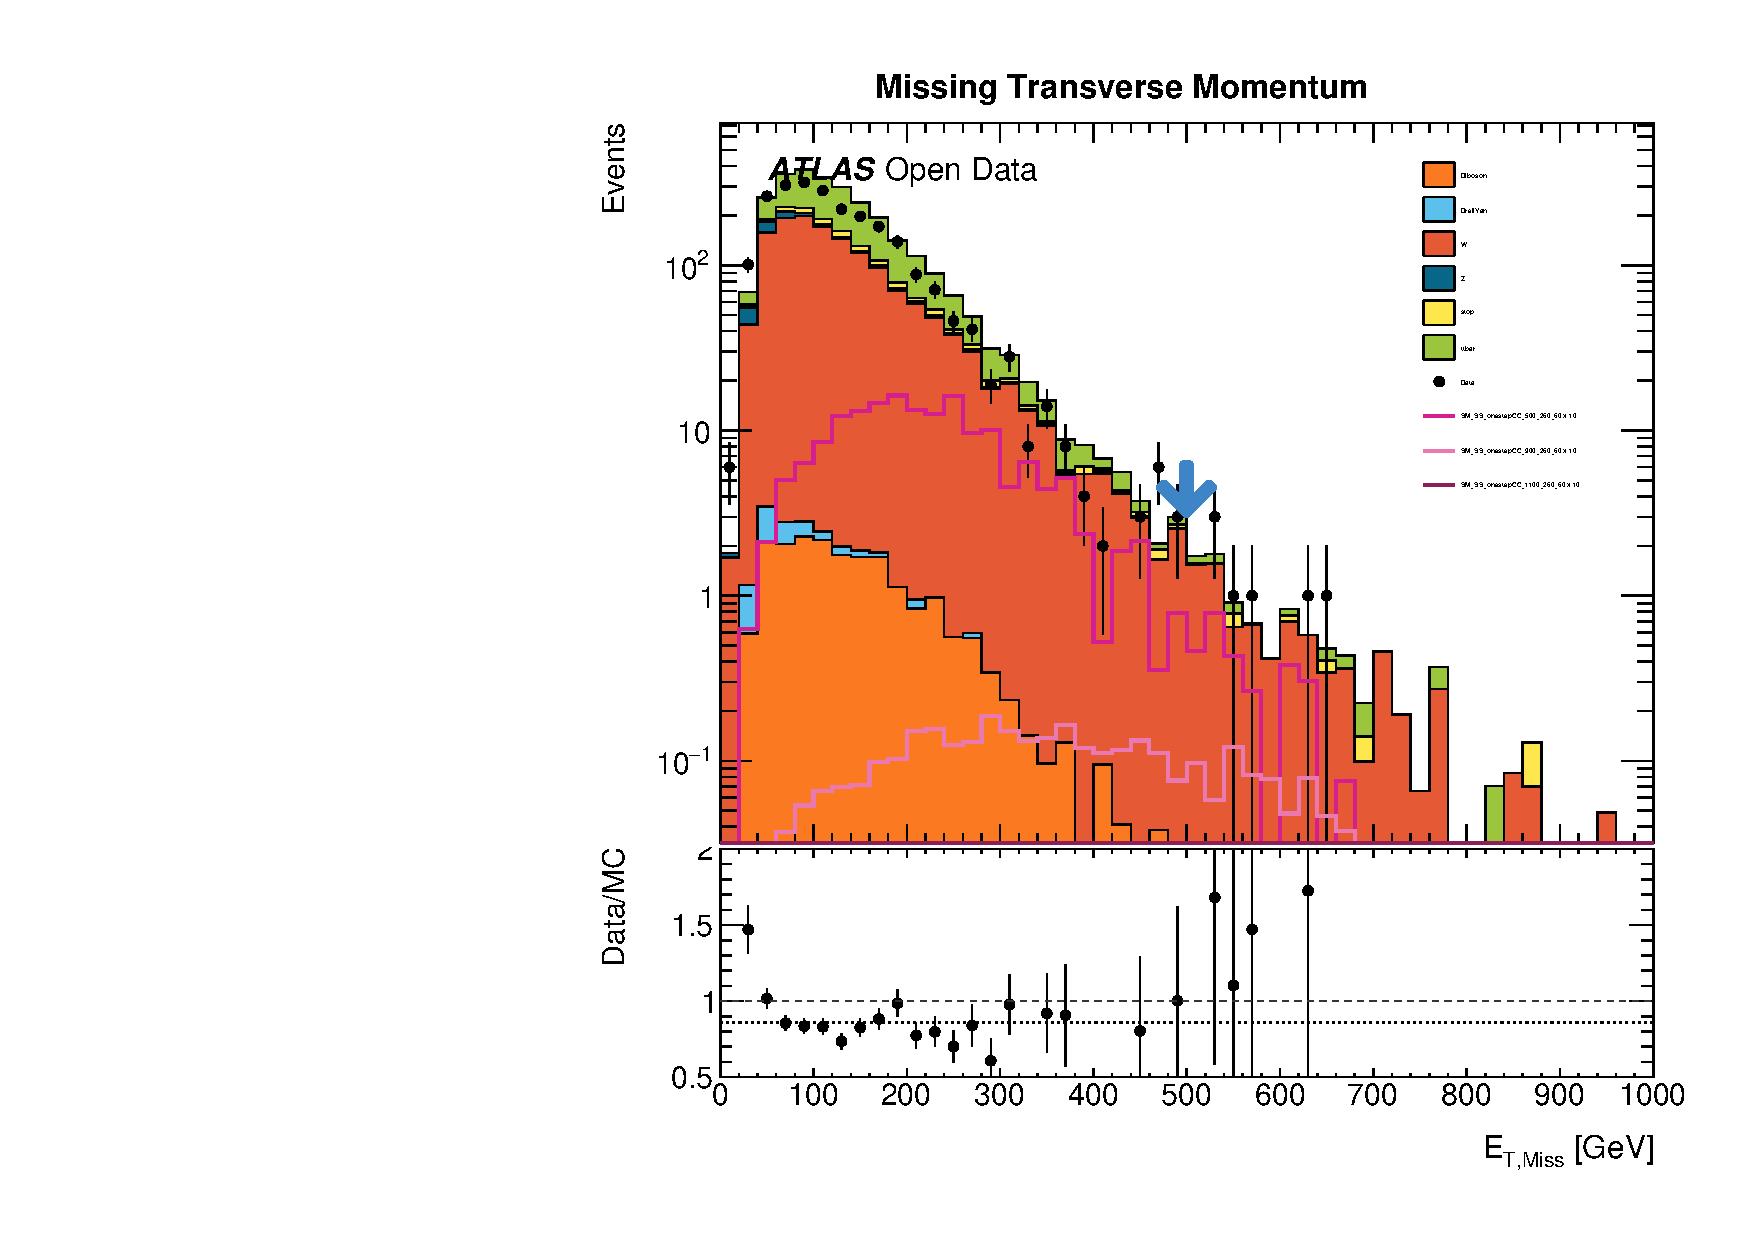
\includegraphics[width=1.\linewidth]{plots/Consider_etmiss_mt150/cropped_etmiss-1_edited.pdf}
\end{minipage}

\caption{Histograms from simulation with standard cuts, and cuts (5-8) in Tab. (\ref{tab::signal cuts}). The blue arrows indicate the $E_{T \text{ miss}}$ cut at $500$ GeV.}
\label{fig:: etmiss hist}
\end{figure}

\begin{figure}[H]
\centering

\begin{minipage}{.5\textwidth}
  \centering
  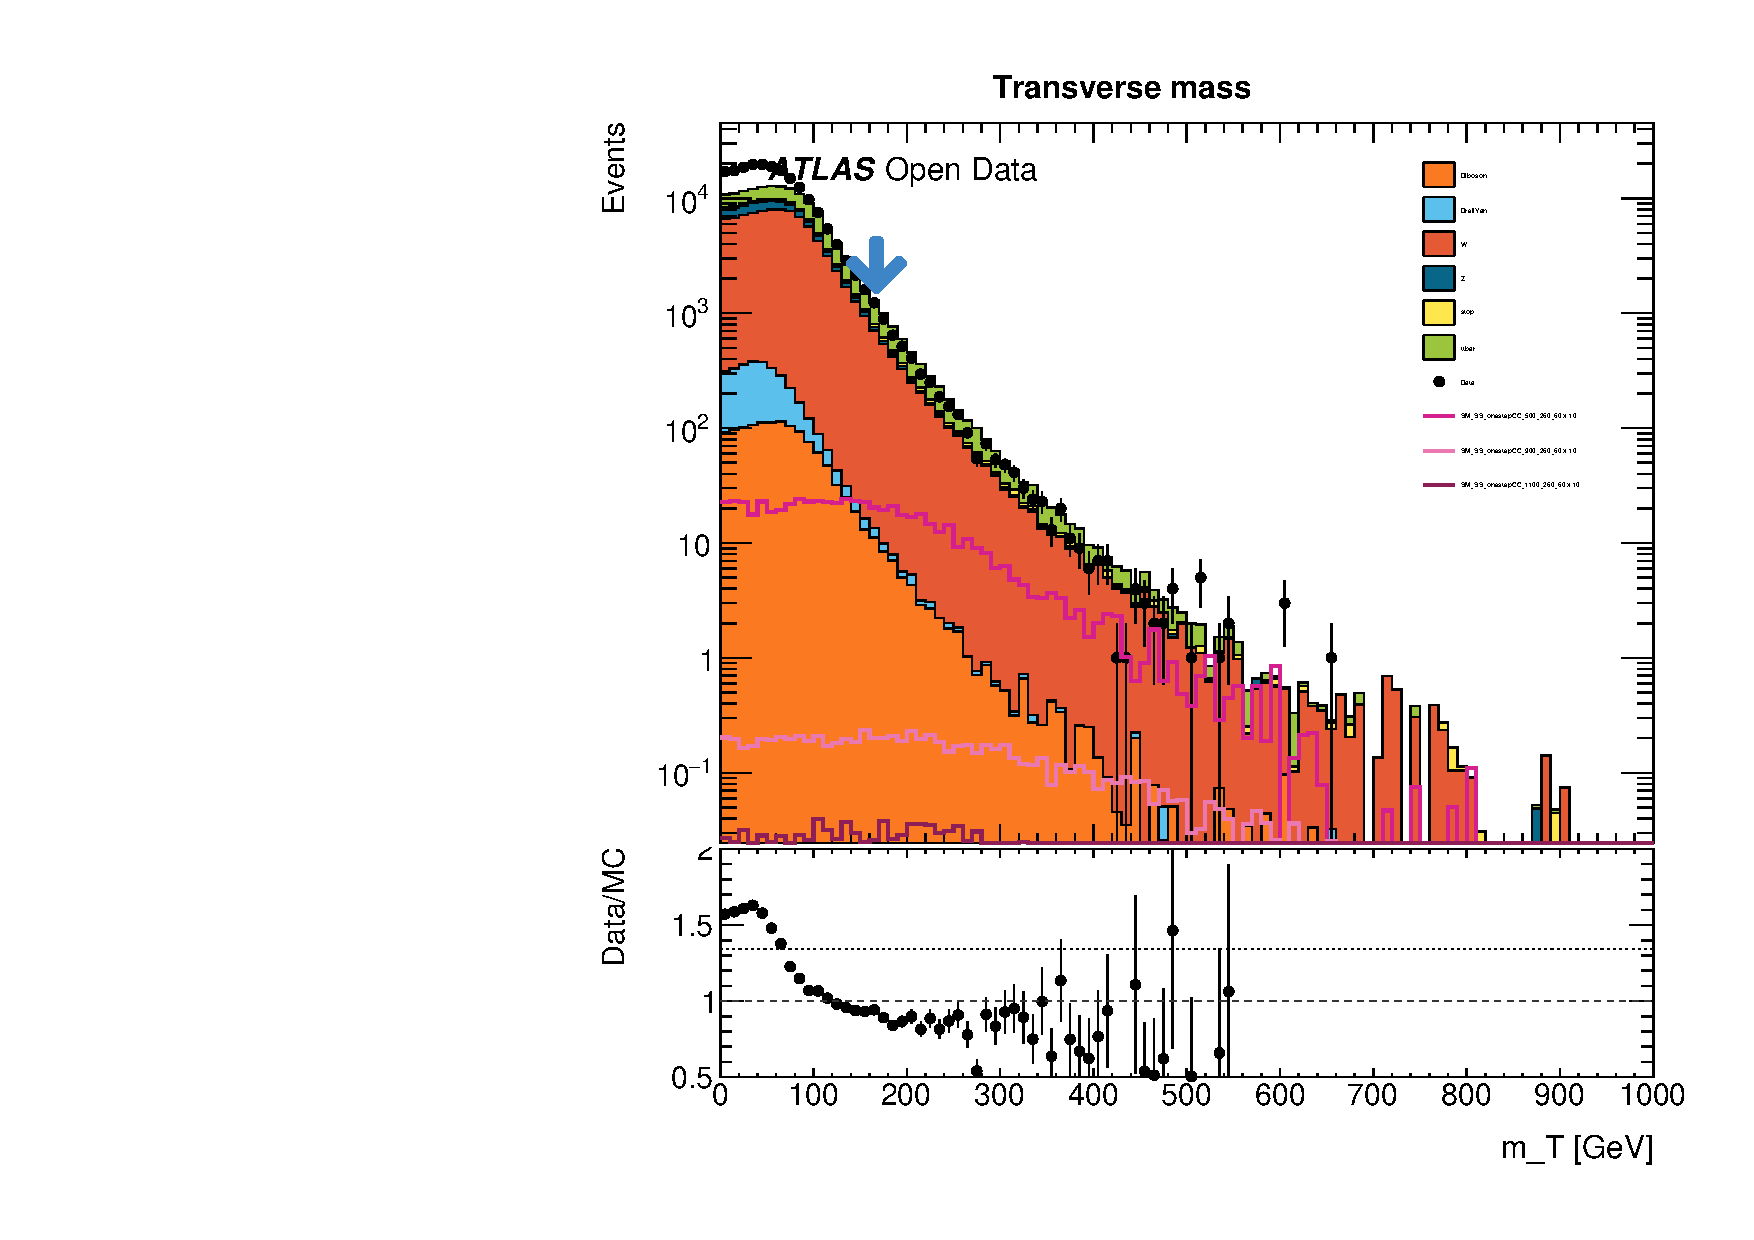
\includegraphics[width=1.\linewidth]{plots/Standard_Cut/cropped_mt_edited.pdf}
\end{minipage}%
\begin{minipage}{.5\textwidth}
  \centering
  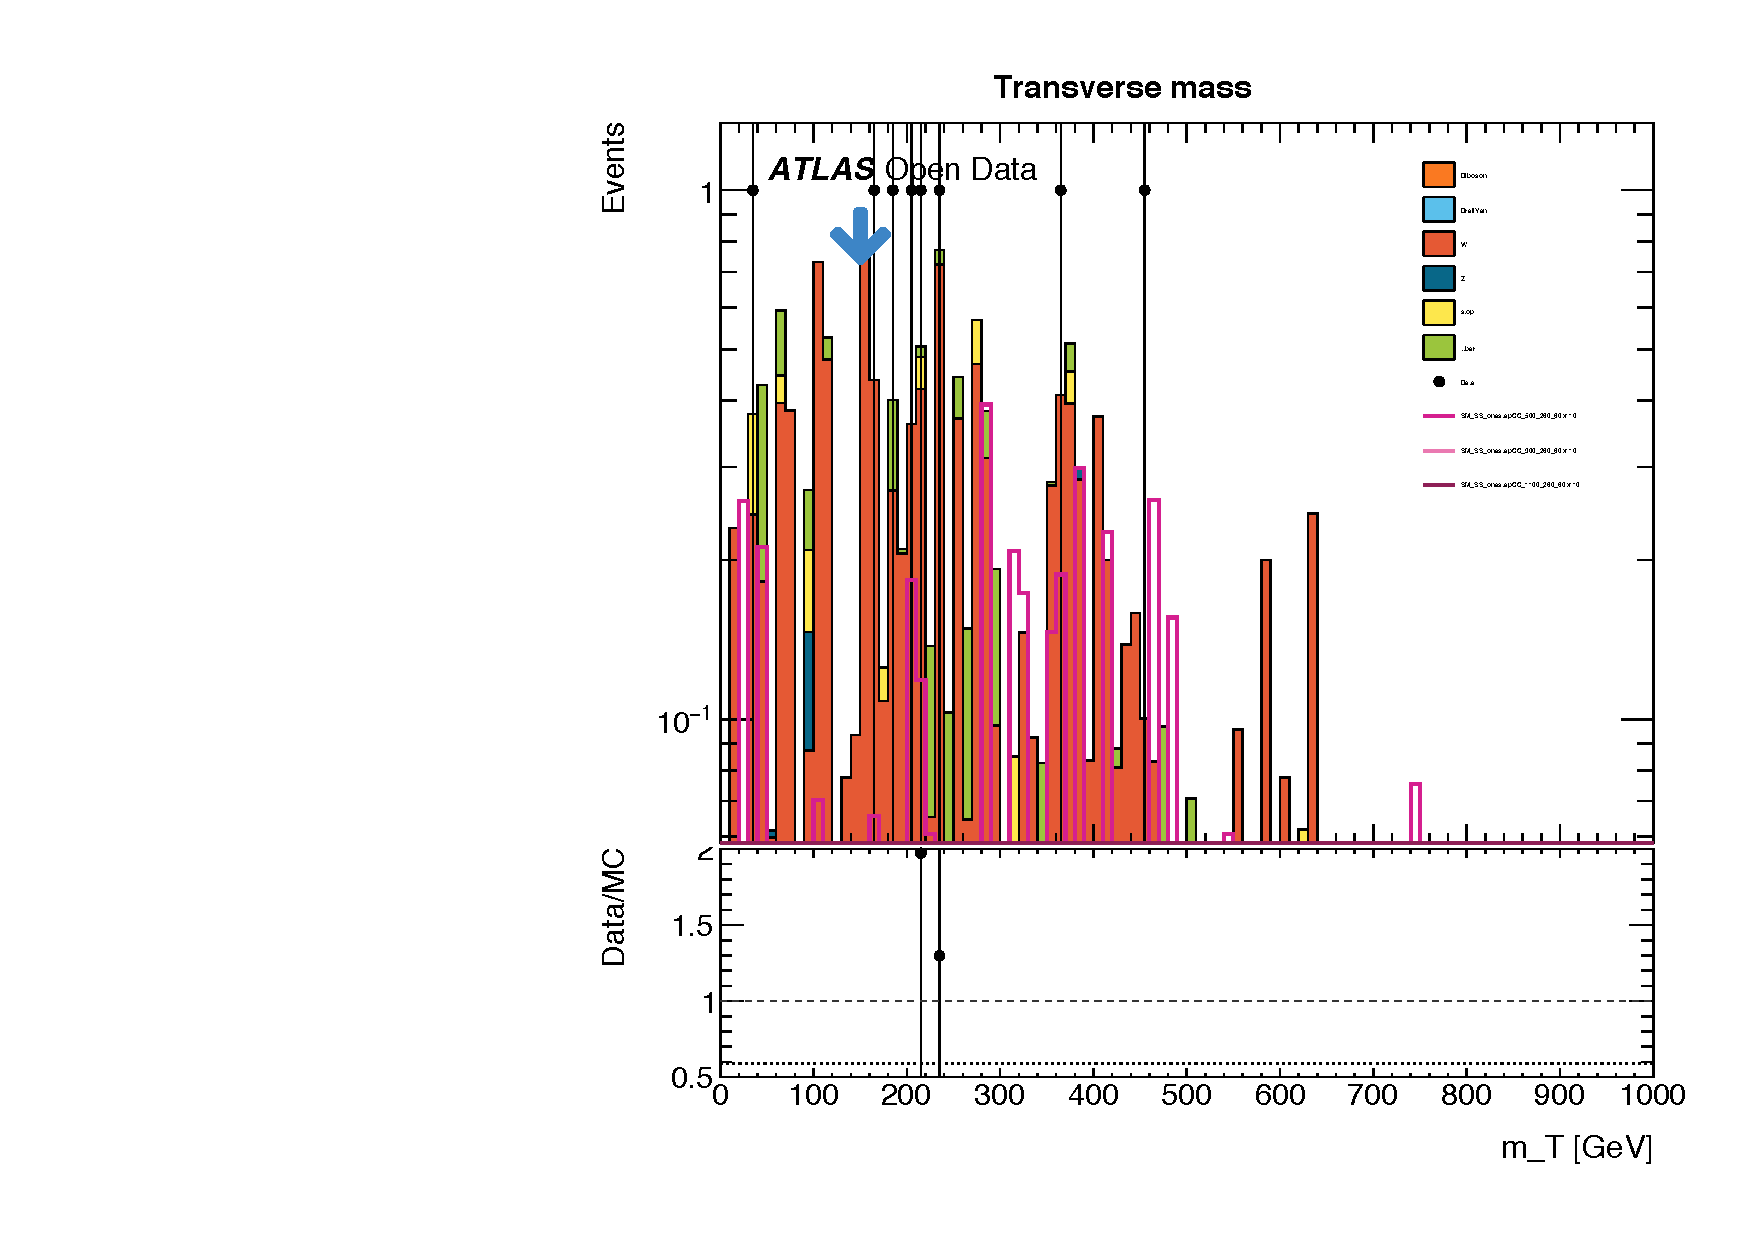
\includegraphics[width=1.\linewidth]{plots/Consider_mt_etmiss500/cropped_mt-2.pdf}
\end{minipage}

\caption{Histograms from simulation with standard cuts, and cuts (5-8) in Tab. (\ref{tab::signal cuts}). The blue arrows indicate the $m_T$ cut at $150$ GeV.}
\label{fig:: mt hist}
\end{figure}

\section*{Conclusion}
\begin{flushleft}
No significant signal was detected, which is not surprising considering how low the cross section is for the desired process. The expected Z-value at $1$ fb$^{-1}$ was not high enough to exclude any masses, but at $20$ fb$^{-1}$ a squark mass of $500$ GeV is excluded, which fits well with \cite{carquin2015search}. However, the cross section for squark production increases with center-of-mass energy as seen in Fig. (\ref{fig:: results LO varying mg mq}), so there may be hope for discovering something at higher energy runs and with higher luminosity.
\end{flushleft}












\pagebreak


\section*{Appendix A}
\subsection*{Feynman rules}
\begin{flushleft}
The following Feynman rules are from \cite{ellis2003qcd} and \cite{beenakker1997squark}. External quarks and squarks
\begin{align*}
\begin{tikzpicture}
\begin{feynman}
\vertex (s); \vertex [right=of s, dot] (p) {};
\diagram{(s) -- [charged scalar] (p)};
\end{feynman}
\end{tikzpicture}
= 1,
\begin{tikzpicture}
\begin{feynman}
\vertex (s); \vertex [right=of s, dot] (p) {};
\diagram{(p) -- [charged scalar] (s)};
\end{feynman}
\end{tikzpicture}
= 1,
\begin{tikzpicture}
\begin{feynman}
\vertex (s); \vertex [right=of s, dot] (p) {};
\diagram{(s) -- [fermion, momentum] (p)};
\end{feynman}
\end{tikzpicture} = u(P),
\begin{tikzpicture}
\begin{feynman}
\vertex (s); \vertex [left=of s, dot] (p) {};
\diagram{(s) -- [fermion] (p), (p) --[momentum] (s)};
\end{feynman}
\end{tikzpicture} = \bar{v}(P).
\end{align*}
Propagator
\begin{align*}
\begin{tikzpicture}
\begin{feynman}
\vertex (s) {a}; \vertex [right=of s] (p) {b};
\diagram{(s) -- [fermion] (p) --[gluon] (s)};
\end{feynman}
\end{tikzpicture} = \delta^{ab} \frac{i}{\cancel{p}-m_{\tilde{g}}},
\begin{tikzpicture}
\begin{feynman}
\vertex (p1) {a}; \vertex [below right=of p1] (p); \vertex [below left=of p] (p2) {i}; \vertex [right=of p] (s);
\diagram{(p1) --[fermion] (p) --[gluon] (p1), (p2) --[fermion] (p), (p) -- [scalar, edge label={j}](s) };
\end{feynman}
\end{tikzpicture} = - i \sqrt{2} g P_{L/R} (t_a)^{ij},
\end{align*}
where the small arrows indicate the reading direction.
\end{flushleft}


\section*{Appendix B}
\subsection*{Calculation of cross section}

\begin{flushleft}
The matrix elements clearly has a contribution from the $t$-channel, the $u$-channel and cross terms. These again give different contributions for different squark handedness. The three contributions will be considered separately, and combined at the end of the calculation.
\end{flushleft}
\subsubsection*{Pure $t$-channel}
\begin{flushleft}
The matrix element is
\begin{align*}
i \mathcal{M} &= \bar{v} (k_1) \Big( -i \sqrt{2} g P (t_a)^{ij}\Big) \times \delta^{ab} \frac{i}{\cancel{p} - m_{\tilde{g}}} \times \Big( -i \sqrt{2} gP'(t_b)^{lk} \Big) \times u(k_2)\\
&= - \frac{i 2 g^2}{p^2 - m_{\tilde{g}}^2 + i \epsilon}\big( \bar{v} (k_1)  P (t_a)^{ij}(\cancel{p} + m_{\tilde{g}}) P'(t^a)^{lk} u(k_2) \big)\\
&= - (t_a)^{ij}(t^a)^{lk} \times \frac{i 2 g^2}{t_g^2} \times  \bar{v} (k_1)  P (\cancel{p} + m_{\tilde{g}}) P' u(k_2) ,
\end{align*}
where the color factor has been factored out. The charge conjugate becomes
\begin{align*}
i \mathcal{\bar{M}} & = (t_a)^{ij}(t^a)^{lk} \times \frac{i 2 g^2}{t_g^2} \times \bar{u} (k_2)  P (\cancel{p} + m_{\tilde{g}}) P' v(k_1) .
\end{align*}
Some Mandelstam variables have been used to clean up the expresson; $t= p^2 = (k_2 - p_2)^2$, $t_g = t - m_{\tilde{g}}^2$. The matrix element squared is then
\begin{align*}
|\mathcal{M}_t|^2 &=  (t_a)^{ij} (t^a)^{lk} (t_b)^{mn} (t^b)^{op} \times \frac{4 g^4}{t_g^2}
\big( \bar{v} (k_1)  P (\cancel{p} + m_{\tilde{g}}) P' u(k_2) \big)
\big( \bar{u} (k_2)  P (\cancel{p} + m_{\tilde{g}}) P' v(k_1) \big).
\end{align*}
\end{flushleft}
Now average over spin
\begin{align*}
\sum |\mathcal{M}_t|^2 &=A_{color, t} \times  \frac{4 g^4}{t_g^2} \text{tr} \big[
(\cancel{k}_1 - m_q)  P (\cancel{p} + m_{\tilde{g}}) P' (\cancel{k}_2 + m_q)  P (\cancel{p} + m_{\tilde{g}}) P' \big],
\end{align*}
where $A_{color, t}= (t_a)^{ij} (t^a)^{lk} (t_b)^{mn} (t^b)^{op}$. Since the quark mass is small compared to $m_g$, $m_{\tilde{q}}$ and $m_{\tilde{g}}$, we set $m_q=0$ and obtain
\begin{align*}
\sum |\mathcal{M}|^2 &= A_{color, t} \times \frac{4 g^4}{t_g^2} \text{tr} \big[ 
\cancel{k}_1 P (\cancel{p} + m_{\tilde{g}}) P' \cancel{k}_2 P (\cancel{p} + m_{\tilde{g}}) P' \big]\\
\end{align*}
At this point we need to consider the different combinations of chiralities. The traces for the different cases are
\begin{center}
\textit{Different chiralities }$P=P_{R/L}$, $P'=P_{L/R}$
\end{center}
\begin{align*}
\text{tr} \big[ 
\cancel{k}_1 P_{R/L} (\cancel{p} + m_{\tilde{g}}) P_{L/R} \cancel{k}_2 P_{R/L} (\cancel{p} + m_{\tilde{g}}) P_{L/R} \big]=& \text{tr} \big[ 
\cancel{k}_1 P_{R/L} (\cancel{p} + m_{\tilde{g}}) P_{L/R} \cancel{k}_2(\cancel{p} + m_{\tilde{g}}) P_{L/R} \big] \\
=& \text{tr} \big[ 
\cancel{k}_1 P_{R/L} \cancel{p} P_{L/R} \cancel{k}_2 \cancel{p} P_{L/R}
+ m_{\tilde{g}} \cancel{k}_1 P_{R/L} \cancel{p} P_{L/R} \cancel{k}_2  P_{L/R}\\
&+ m_{\tilde{g}} \cancel{k}_1 P_{R/L}  P_{L/R} \cancel{k}_2\cancel{p} P_{L/R}
+ m_{\tilde{g}}^2 \cancel{k}_1 P_{R/L} P_{L/R} \cancel{k}_2  P_{L/R} \big]\\
=& \text{tr} \big[ P_{L/R} 
\cancel{k}_1 \cancel{p} \cancel{k}_2 \cancel{p}  \big]\\
&= \text{tr} \big[
 P_{R/L}[2 p \cdot k \cancel{k}_1 \cancel{p} - p^2\cancel{k}_1 \cancel{k}_2 ]  \big]\\
 &=\frac{1}{2} \text{tr} \big[
2 p \cdot k_2 \cancel{k}_1 \cancel{p} - p^2\cancel{k}_1 \cancel{k}_2 \big]\\
&= 2 \big(
2 (p \cdot k_2) (k_1 \cdot p) - p^2 (k_1 \cdot k_2)\big)
\end{align*}
where the middle terms dissappear because they contain an odd number of $\gamma^{\mu}$, and the terms with an even number of $\gamma^{\mu}$ in the last term cancel out.
\begin{center}
\textit{Equal chiralities} $P=P_{R/L}$, $P'=P_{R/L}$
\end{center}
\begin{align*}
\text{tr} \big[ 
\cancel{k}_1 P_{R/L} (\cancel{p} + m_{\tilde{g}}) P_{R/L} \cancel{k}_2 P_{R/L} (\cancel{p} + m_{\tilde{g}}) P_{R/L} \big]=& \text{tr} \big[ 
\cancel{k}_1 P_{R/L} \cancel{p} P_{R/L} \cancel{k}_2 P_{R/L} \cancel{p}  P_{R/L}
+ m_{\tilde{g}} \cancel{k}_1 P_{R/L} \cancel{p} P_{R/L} \cancel{k}_2 P_{R/L} P_{R/L}\\
&+ m_{\tilde{g}} \cancel{k}_1 P_{R/L}P_{R/L} \cancel{k}_2 P_{R/L} \cancel{p} P_{R/L}
+ m_{\tilde{g}}^2 \cancel{k}_1 P_{R/L}  P_{R/L} \cancel{k}_2 P_{R/L} P_{R/L} \big]\\
&= \frac{1}{4} \text{tr} \big[ m_{\tilde{g}}^2 \cancel{k}_1 \big( 1 \pm \gamma^5 \big) \cancel{k}_2 \big( 1 \pm \gamma^5 \big)\big]\\
&= \frac{1}{2} \text{tr} \big[ m_{\tilde{g}}^2 \cancel{k}_1 \cancel{k}_2\big] =  m_{\tilde{g}}^2 (2 k_1 \cdot k_2)
\end{align*}
where we've used that $P_{R/L}P_{R/L} = P_{R/L}$, $(\gamma^5)^2 = 1$ and $\text{tr}[\gamma^5 \gamma^{\mu} \gamma^{\nu}]=0$. Now clean up using the following Mandelstam variables
\begin{multicols}{3}

\begin{align*}
s &= (k_1 + k_2)^2 = 2 k_1 \cdot k_2\\
t &= (k_2-p_2)^2 = m_{\tilde{q}}^2 - 2 (k_2 \cdot p_2),\\
u &= (k_1 - p_2)^2 = m_{\tilde{q}}^2 - 2 (k_1 \cdot p_2),
\end{align*}

\begin{align*}
t_1 &= (k_2-p_2)^2 - m_{\tilde{q}}^2,\\
u_1 &= (k_1-p_2)^2 - m_{\tilde{q}}^2,
\end{align*}

\begin{align*}
t_g &= (k_2-p_2)^2 - m_{\tilde{g}}^2,\\
u_g &= (k_1-p_2)^2 - m_{\tilde{g}}^2.
\end{align*}

\end{multicols}

The expression can now be simplified
\begin{align*}
&2(2 (p \cdot k_2) (k_1 \cdot p) - p^2 (k_1 \cdot k_2) ) + 2m_{\tilde{g}}^2 (k_1 \cdot k_2)\\ &= 4((k_2 - p_2) \cdot k_2) (k_1 \cdot (k_2-p_2)) - 2t (k_1 \cdot k_2) + 2m_{\tilde{g}}^2 (k_1 \cdot k_2)\\
&=-4(p_2 \cdot k_2)(k_1 \cdot k_2 - k_1 \cdot p_2) - 2t(k_1 \cdot k_2) + 2m_{\tilde{g}}^2 (k_1 \cdot k_2)\\
&= -4 (p_2 \cdot k_2)(k_1 \cdot k_2) + 4(p_2 \cdot k_2)(k_1 \cdot p_2) - 2t (k_1 \cdot k_2) + 2m_{\tilde{g}}^2 (k_1 \cdot k_2)\\
&= 4 \frac{1}{2}(t-m_{\tilde{q}}^2)\cdot \frac{1}{2}s + 4 \frac{1}{2}(t-m_{\tilde{q}}^2)\cdot \frac{1}{2}(u-m_{\tilde{q}}^2)-  ts + m_{\tilde{g}}^2 s\\
&= t_1s+t_1u_1 -ts\\
&= t_1u_1 - s(t-t_1) m_{\tilde{g}}^2 s = 2 \big[t_1u_1 -s(m_{\tilde{q}}^2 - m_{\tilde{g}}^2) \big].
\end{align*}
Note that for equal quark flavors, the two possibilities for different chiralities are in fact equal, and so there should be a factor of $1/2$ there. Now put this back into the expression 
\begin{align*}
\sum |\mathcal{M}|^2 &=   (t_a)^{ij} (t^a)^{lk} (t_b)^{mn} (t^b)^{op}  \times\frac{4 g^4}{t_g^2} \Big[\delta_{ij} \big(\frac{1}{2}(t_1u_1 -sm_{\tilde{q}}^2)+  sm_{\tilde{g}}^2 \big) + (1-\delta_{ij})\big(t_1u_1 -s(m_{\tilde{q}}^2- m_{\tilde{g}}^2) \big)\Big].
\end{align*}
We still need to sum over colors, and we use the relation \cite{ellis2003qcd}
\begin{align*}
\sum_a (t^a)_{ij}(t^a)_{lk} = \frac{1}{2} \big(\delta_{ik} \delta_{lj} - \frac{1}{N} \delta_{ij} \delta_{lk} \big).
\end{align*}
Combine the factors
\begin{align*}
(t^a)^{ij}(t_a)^{kl}(t^b)_{ij}(t_b)^{kl} &= \frac{1}{4} 
\big(\delta_{ik} \delta_{lj} - \frac{1}{N} \delta_{ij} \delta_{lk} \big)
\big(\delta^{ik} \delta^{lj} - \frac{1}{N} \delta^{ij} \delta^{lk} \big)\\
&= \frac{1}{4} \Big(\delta_{ik} \delta_{lj}\big(\delta^{ik} \delta^{lj} - \frac{1}{N} \delta^{ij} \delta^{lk} \big) - \frac{1}{N} \delta_{ij} \delta_{lk}\big(\delta^{ik} \delta^{lj} - \frac{1}{N} \delta^{ij} \delta^{lk} \big) \Big)\\
&= \frac{1}{4} \Big(\big(N N - \frac{1}{N} N \big)  - \frac{1}{N} \big(N - \frac{1}{N} N N \big) \Big)\\
&= \frac{1}{4} (N^2 - 1) = \frac{1}{2}NC_F,
\end{align*}
where we have defined $C_F = \frac{N^2 -1}{2}$. Adding a factor $2$ because we are summing over the different chiralities, the full expression for the $t$-channel is then
\begin{align*}
\sum |\mathcal{M}_t|^2 &= NC_F \frac{4g^4}{t_g^2} \Big[ \delta_{ij} \big(\frac{1}{2}(t_1u_1-sm_{\tilde{q}}^2) + sm_{\tilde{g}}^2 \big) + (1-\delta_{ij}) \big(t_1u_s - s(m_{\tilde{q}}^2 - m_{\tilde{g}}^2) \big)\Big]
\end{align*}

\subsubsection*{Pure $u$-channel}
\begin{flushleft}
The expression for the $u$-channel diagram is identical, except the exchange of $t_g^2 \rightarrow u_g^2$ and the color factor must be calculated again,
\begin{align*}
\sum |\mathcal{M}_u|^2 = \delta_{ij} A^2_{color, u} \frac{4 g^4}{u_g^2} [\frac{1}{2}( u_1 t_1 - sm_{\tilde{q}}^2) +s m_{\tilde{g}}^2)]. 
\end{align*}
The color factor becomes
\begin{align*}
\sum_{a,b}(t^a)^{ik}(t_a)^{jl}(t^b)_{ik}(t_b)_{jl} &= \frac{1}{4}(\delta_{ij}\delta_{lk}-\frac{1}{N}\delta_{ik}\delta_{jl})(\delta^{ij}\delta^{lk}-\frac{1}{N}\delta^{ik}\delta^{jl})\\
&= \frac{1}{4} \big(\delta_{ij}\delta_{lk}(\delta^{ij}\delta^{lk}-\frac{1}{N}\delta^{ik}\delta^{jl}) -\frac{1}{N}\delta_{ik}\delta_{jl}(\delta^{ij}\delta^{lk}-\frac{1}{N}\delta^{ik}\delta^{jl}) \big)\\
&= \frac{1}{4} \big(\delta_{ij}\delta^{ij} \delta_{kl} \delta^{kl} - \frac{1}{N} \delta^{jk}\delta_{kj} - \frac{1}{N} \delta^{jk}\delta_{jk} + \frac{1}{N^2} \delta_{ik} \delta^{ik} \delta_{jl} \delta^{jl} \big)\\
&= \frac{1}{4} (N^2-1).
\end{align*}
Since we are summing over the different parity combinations we add a factor of $2$, and the total $u$-channel contribution becomes
\begin{align*}
\sum |\mathcal{M}_u|^2 &= \delta_{ij} NC_F 4g^4 [\frac{1}{2}( u_1 t_1 - sm_{\tilde{q}}^2) +s m_{\tilde{g}}^2)]
\end{align*}
\end{flushleft}

\subsubsection*{Cross terms}
\begin{flushleft}
The cross term comes from
\begin{align*}
i \mathcal{M}_{ut} &= A_{color, ut}\frac{-i 2 g^2}{t_g}\big( \bar{v} (k_1)  P (\cancel{p} + m_{\tilde{g}}) P'u(k_2) \big)  \frac{i 2 g^2}{u_g} \big( \bar{u} (k_2)  P (\cancel{p} + m_{\tilde{g}}) P' v(k_1) \big)\\
\sum \mathcal{M}_{ut} &= A_{color, ut} \frac{4 g^4}{u_gt_g}\big( \cancel{k}_1   P (\cancel{k}_2 - \cancel{p}_2 + m_{\tilde{g}}) P'\cancel{k}_2  P (\cancel{k}_2 -\cancel{p}_1 + m_{\tilde{g}}) P' \big)\\
\end{align*}
Average over spins
\begin{align*}
\sum  \mathcal{M}_{ut} &=  A_{color, ut} \frac{4 g^4}{u_gt_g}\big( \text{tr} \big[ \cancel{k}_1 P_{L/R} (\cancel{k}_2 - \cancel{p}_2)P_{R/L} \cancel{k}_2(\cancel{k}_2-\cancel{p}_1) \big] + \text{tr} \big[ \cancel{k}_1 m_{\tilde{g}} \cancel{k}_2 m_{g}^2 \big]\big)\\
&= A_{color, ut} \frac{4 g^4}{u_gt_g} \big(
 \text{tr} \big[ \frac{1}{2}\Big(1 - \gamma^5 \Big) \cancel{k}_1 (\cancel{k}_2 - \cancel{p}_2) \cancel{k}_2(\cancel{k}_2-\cancel{p}_1) \big] + \text{tr} \big[\frac{1}{2} m_{\tilde{g}}^2 \cancel{k}_1  \cancel{k}_2\big]
  \big)\\
&= A_{color, ut} \frac{4 g^4}{u_gt_g} \big(
 \frac{1}{2} \text{tr} \big[\Big(1 - \gamma^5 \Big) \big( \cancel{k}_1 \cancel{k}_2 \cancel{k}_2\cancel{p}_2 -  \cancel{k}_1 \cancel{k}_2 \cancel{k}_2\cancel{k}_1 -  \cancel{k}_1 \cancel{p}_2 \cancel{k}_2\cancel{p}_2 +  \cancel{k}_1 \cancel{p}_2 \cancel{k}_2\cancel{k}_1 \big) \big] + \text{tr} \big[\frac{1}{2} m_{\tilde{g}}^2 \cancel{k}_1  \cancel{k}_2\big]
  \big)\\
&= A_{color, ut} \frac{4 g^4}{u_gt_g} \big(
 \frac{1}{2} \text{tr} \big[\Big(1 - \gamma^5 \Big) \big(k_2^2 (\cancel{k}_1 \cancel{p}_2 -  \cancel{k}_1 \cancel{k}_1)
  -  \cancel{k}_1 (2 p_2 \cdot k_2 -  \cancel{k}_2\cancel{p}_2)\cancel{p}_2 +  (2k_1 \cdot p_2 - \cancel{p}_2 \cancel{k}_1 )(2k_2 \cdot k_1 - \cancel{k}_1\cancel{k}_2) \big) \big] + \text{tr} \big[\frac{1}{2} m_{\tilde{g}}^2 \cancel{k}_1  \cancel{k}_2\big]
  \big)\\
 &= A_{color, ut} \frac{4 g^4}{u_gt_g} \big(
 \frac{1}{2} \text{tr} \big[\Big(1 - \gamma^5 \Big) \big(
  -   2 p_2 \cdot k_2\cancel{k}_1\cancel{p}_2 + p_2^2  \cancel{k}_1\cancel{k}_2 \\
&  + (2k_1 \cdot p_2)(2k_2 \cdot k_1) - (2k_1 \cdot p_2)\cancel{k}_1\cancel{k}_2 - \cancel{p}_2 \cancel{k}_1(2k_2 \cdot k_1) + k_1^2\cancel{p}_2 \cancel{k}_2 \big) \big] + \frac{1}{2} m_{\tilde{g}}^2 \cancel{k}_1  \cancel{k}_2\big]
  \big)\\
  &=  A_{color, ut} \frac{4 g^4}{u_gt_g} \big(
  -   (2 p_2 \cdot k_2)(2k_1 \cdot p_2) + p_2^2  (2k_1 \cdot k_2) \\
&  + 2(2k_1 \cdot p_2)(2k_2 \cdot k_1) - (2k_1 \cdot p_2)(2k_1 \cdot k_2) - (2 p_2 \cdot k_1)(2k_2 \cdot k_1) 
+  m_{\tilde{g}}^2 (2k_1 \cdot k_2) 
  \big)\\
&=  A_{color, ut} \frac{4 g^4}{u_gt_g} \big(
  -   t_1 u_1 + p_2^2  s  + 2(-u_1)s + u_1s +u_1s 
+  m_{\tilde{g}}^2 s
  \big)\\
  &=  A_{color, ut} \frac{4 g^4}{u_gt_g} \big(
  -   t_1 u_1 + m_{\tilde{q}}^2 s 
+  m_{\tilde{g}}^2 s
  \big)\\
\end{align*}
The other counter term is similar, but yields a different order
\begin{align*}
\sum i \mathcal{M}_{tu} &= A_{color, tu} \frac{4 g^4}{u_gt_g}\big( \cancel{k}_1   P (\cancel{k}_2 - \cancel{p}_1 + m_{\tilde{g}}) P'\cancel{k}_2  P (\cancel{k}_2 -\cancel{p}_2 + m_{\tilde{g}}) P' \big)\\
&= A_{color, ut} \frac{4 g^4}{u_gt_g} \big(
 \text{tr} \big[ \frac{1}{2}\Big(1 - \gamma^5 \Big) \cancel{k}_1 (\cancel{k}_2 - \cancel{p}_1) \cancel{k}_2(\cancel{k}_2-\cancel{p}_2) \big] + \text{tr} \big[\frac{1}{2} m_{\tilde{g}}^2 \cancel{k}_1  \cancel{k}_2\big]
  \big)\\
  &= A_{color, ut} \frac{4 g^4}{u_gt_g} \big(
 \frac{1}{2} \text{tr} \big[\Big(1 - \gamma^5 \Big) \cancel{k}_1 (\cancel{p}_2 - \cancel{k}_1 - \cancel{k}_2) \cancel{k}_2\cancel{p}_2  \big] + \text{tr} \big[\frac{1}{2} m_{\tilde{g}}^2 \cancel{k}_1  \cancel{k}_2\big]
  \big)\\
  &= A_{color, ut} \frac{4 g^4}{u_gt_g} \big(
 \frac{1}{2} \text{tr} \big[\Big(1 - \gamma^5 \Big) \big( \cancel{k}_1 \cancel{p}_2 \cancel{k}_2\cancel{p}_2 - \cancel{k}_1\cancel{k}_1 \cancel{k}_2\cancel{p}_2 - \cancel{k}_1 \cancel{k}_2 \cancel{k}_2\cancel{p}_2  \big)\big] + \text{tr} \big[\frac{1}{2} m_{\tilde{g}}^2 \cancel{k}_1  \cancel{k}_2\big]
  \big)\\
  &= A_{color, ut} \frac{4 g^4}{u_gt_g} \big(
 \frac{1}{2} \text{tr} \big[\Big(1 - \gamma^5 \Big) \big( \cancel{k}_1 \cancel{p}_2 (2 (k_2 \cdot p_2)- \cancel{p}_2\cancel{k}_2)  \big)\big] + \text{tr} \big[\frac{1}{2} m_{\tilde{g}}^2 \cancel{k}_1  \cancel{k}_2\big]
  \big)\\
&= A_{color, ut} \frac{4 g^4}{u_gt_g} \big(
 \frac{1}{2} \text{tr} \big[ \cancel{k}_1 \cancel{p}_2 (2 k_2 \cdot p_2)- p_2^2\cancel{k}_1 \cancel{k}_2)  \big] + \text{tr} \big[\frac{1}{2} m_{\tilde{g}}^2 \cancel{k}_1  \cancel{k}_2\big]
  \big)\\
  &=  A_{color, ut} \frac{4 g^4}{u_gt_g} \big(
(2k_1 \cdot p_2) (2 k_2 \cdot p_2)- p_2^2(2 k_1 \cdot k_2)  \big] + m_{\tilde{g}}^2(2 k_1 \cdot k_2)
  \big)\\
  &= A_{color, ut} \frac{4 g^4}{u_gt_g} \big(
u_1t_1- m_{\tilde{q}}^2s + m_{\tilde{g}}^2s
  \big).
\end{align*}
Adding the counter terms, noting that this term only contributes when the quark flavors are the same, then gives 
\begin{align*}
\sum |\mathcal{M}_{ut+tu}| &= A_{color, ut} \frac{4 g^4}{u_gt_g} \delta_{ij}\big(2 m_{\tilde{g}}^2s   \big).
\end{align*}
The color factor is
\begin{align*}
\sum_{a,b}(t^a)^{ij}(t_a)^{kl}(t^b)_{ik}(t_b)_{jl} &= \frac{1}{4}(\delta_{ik}\delta_{lj}-\frac{1}{N}\delta_{ij}\delta_{kl})(\delta^{ij}\delta^{lk}-\frac{1}{N}\delta^{ik}\delta^{jl})\\
 &= \frac{1}{4} \big(\delta_{ik}\delta_{lj}(\delta^{ij}\delta^{lk}-\frac{1}{N}\delta^{ik}\delta^{jl}) -\frac{1}{N}\delta_{ij}\delta_{kl}(\delta^{ij}\delta^{lk}-\frac{1}{N}\delta^{ik}\delta^{jl})\big)\\
 &= \frac{1}{4} \big(N-\frac{1}{N}N^2 - \frac{1}{N}N^2 + \frac{1}{N^2} N \big)\\
 &= - \frac{1}{4}\big(N -\frac{1}{N} \big)\\
 &= - \frac{1}{2}C_F
\end{align*}
\end{flushleft}

\begin{flushleft}
Now, combining the terms, noting that the $u$-channel will only contribute for same-flavour quarks, we find
\begin{align*}
\sum |\mathcal{M}|^2 =& \delta_{ij}  \Bigg[2 g^4NC_F(u_1t_1-sm_{\tilde{q}}^2) \big( \frac{1}{t_g^2} + \frac{1}{u_g^2} \big) + 4 g^4 sm_{\tilde{g}}^2 \Big( NC_F \big(\frac{1}{t_g^2} + \frac{1}{u_g^2}\big) -2C_F\frac{1}{u_gt_g} \Big) \Bigg]\\
&+ (1-\delta_{ij})\Bigg[4g^4NC_F  \frac{u_1t_1-s(m_{\tilde{g}}^2-m_{\tilde{g}}^2)}{t_g^2} \Bigg].
\end{align*}
\end{flushleft}



\bibliographystyle{plain}
\bibliography{susy_project}

\end{document}
